% DSB300 Capstone, Group 15. Compile with pdfLaTeX (Overleaf default).
\documentclass[11pt,a4paper]{article}
\usepackage[T1]{fontenc}
\usepackage[utf8]{inputenc}
\usepackage{lmodern}
\usepackage[margin=2.5cm]{geometry}
\usepackage{amsmath,amssymb}
\usepackage{graphicx}
\usepackage{booktabs}
\usepackage{makecell}
\usepackage[labelfont=bf,labelsep=period,justification=raggedright,singlelinecheck=false,skip=6pt]{caption}
\usepackage[hidelinks]{hyperref}

\setlength{\parindent}{0pt}
\setlength{\parskip}{0.6em}
\setcounter{secnumdepth}{0}  % unnumbered headings, as in the Word version
\providecommand{\tightlist}{\setlength{\itemsep}{0pt}\setlength{\parskip}{0pt}}
\newcommand{\tablenote}[1]{\par\smallskip\parbox{\linewidth}{\footnotesize\textit{Note.} #1}}

\begin{document}

\hypersetup{pageanchor=false}
\begin{titlepage}
\centering
{\large\bfseries Queensland University of Technology\par}
\vspace{0.3em}
{DSB300 Data Science Capstone\par}
\vspace{4cm}
{\Huge\bfseries Journal Citation Analytics\par}
\vspace{0.8em}
{\Large How can FSR attract more citations?\par}
\vspace{3cm}
{\bfseries Industry Partner\par}
Academy of Financial Services (AFS)\par
\vspace{1em}
{\bfseries Partner Supervisors\par}
Shawn Brayman, Dr Norah Feng\par
\vspace{3cm}
{\bfseries Prepared by Group 15\par}
Gia Tran\par
Huy Nhat Minh Nguyen\par
Thuy Huyen Tran, n11991615\par
Shiqi Guan\par
\vfill
{\bfseries Date\par}
23 October 2026\par
\end{titlepage}
\hypersetup{pageanchor=true}

\section{Executive summary}\label{executive-summary}

\textit{[To be completed.]}
% Template guidance (1 to 2 pages, max 3 pages). Use plots to make your point clearly and succinctly
% where appropriate. This document must: summarise the problem and context; summarise the reviewed
% literature and justify the chosen method; summarise the data and results, clearly communicating the
% validity of the artefact, its explainability and uncertainty where appropriate (e.g. confidence
% intervals, quantitative covariate/feature effects); conclude with a link back to the project
% objectives and any recommendations.

\clearpage

\section{Public executive summary}\label{public-executive-summary}

\textit{[To be completed.]}
% Template guidance (1 to 2 pages, max 3 pages). A sanitised version of the preceding executive summary
% with all commercial-in-confidence labels and/or information removed. This should still attempt to
% capture the key data science context, work and findings that can be released, and should not be just
% a redacted version of the executive summary. You need to get your industry partner to check over your
% public executive summary (only) and include as an attachment to your submission an email from them
% confirming that it does not contain commercial-in-confidence information.

\clearpage

\section{Introduction}\label{introduction}

Academic journal citations are commonly used as an indicator of the visibility, influence, and dissemination of published research. For journal publishers and editorial teams, understanding the factors associated with citation performance can support decisions concerning journal positioning, topic selection, and future publication strategies. However, citation counts are influenced by several factors, including the age of an article, its research topic, and the characteristics of the journal in which it is published. Consequently, raw citation counts alone may not provide a fair basis for comparing articles or journals.

The Academy of Financial Services (AFS) is seeking to improve the citation performance and academic visibility of Financial Services Review (FSR). This project therefore investigates the question: How can FSR attract more citations? To address this question, the study analyses bibliographic metadata obtained from Scopus for articles published in FSR and two related journals, Financial Planning Review (FPR), and the Journal of Financial Counseling and Planning (JFCP). Comparing FSR with these journals provides a broader view of citation patterns within the financial services and financial planning research field.

The analysis examines the distribution of citations across the three journals and considers the effect of publication age, as older articles have had more time to accumulate citations. It also investigates the research topics represented in each journal and their relationship with citation performance. This combination of citation and topic analysis is intended to identify both the factors associated with highly cited articles and potentially influential research areas that may be underrepresented in FSR.

The main objective of the project is to produce evidence-based recommendations that can help AFS strengthen the positioning and citation impact of FSR. The findings may assist the journal's editorial team in identifying promising research themes, understanding their performance relative to comparable journals, and making informed decisions about future calls for papers and editorial priorities.

The project addresses four research questions, each taken up in turn in the Methods, Results and Discussion sections that follow:

\begin{enumerate}
\item[\textbf{A.}] Are citations concentrated among a small number of prolific or well-known authors, and does an author's prior track record predict how their FSR papers perform?
\item[\textbf{B.}] Which research topics are associated with higher citation counts, and where does FSR under-publish relative to its comparators?
\item[\textbf{C.}] Does abstract readability relate to citations in FSR, and does that relationship differ across the three journals?
\item[\textbf{D.}] How many years after publication do FSR papers typically peak, and can the papers that go on to be highly cited be identified early?
\end{enumerate}

\section{Literature review}\label{literature-review}

The relationship between publication characteristics and research impact has been extensively examined in the academic literature. Researchers across multiple disciplines have investigated whether factors related to article content, authorship, and journal characteristics are associated with citation performance. The methodologies they used to examine these relationships also differ across studies, from correlation analysis to regression and more advanced machine-learning approaches. The following section provides an overview of existing literature on citation performance and evaluates the methodologies used, including their strengths and limitations and relevance to the current problem.

As highlighted by Kousha and Thelwall (2024) in their comprehensive review of existing studies, citation impact is not driven by a single factor. The studies reviewed draw on bibliometric data from publications across different research fields. Collectively, they suggest that citation count may be associated with a combination of characteristics related to the paper itself, the authors behind it and journal reputation. These findings are also highly context-dependent, meaning the effects of these factors are not universal and vary across disciplines and journals.

Before the growing use of machine learning and text-mining approaches, researchers primarily relied on traditional statistical methods to investigate factors associated with citation impact. Moreover, these studies often examined specific characteristics of research publications. For example, Gazni (2011) focused on the relationship between abstract readability and citation impact. To investigate this relationship, Gazni measured abstract readability using the Flesch Reading Ease formula and applied correlation analysis to examine its association with scientific impact, using citation counts as a proxy. The study compared readability scores across disciplines and publication years and found that highly cited articles generally received lower readability scores. While this approach is simple, straightforward and computationally efficient, the Flesch Reading Ease formula relies on word and sentence length and does not capture more complex linguistic characteristics or the overall clarity of an abstract. Additionally, the analysis did not account for other confounding factors that may influence citation counts. Thus, the findings do not imply that making an abstract more complex would guarantee that the article receives more citations. The study is directly relevant to the FSR problem, as abstract readability is one of the many factors worth considering when examining what drives citation impact.

Sienkiewicz and Altmann (2016) extended this work by using a more sophisticated analytical technique and more complex textual elements in their analysis. In addition to text length and readability, the authors also assessed lexical difficulty and sentiment variables, such as valence and arousal. Rather than relying on simple correlation, they used quantile regression to assess how these relationships shifted across papers with various levels of citation impact. The analysis showed that some textual characteristics behaved differently with low, medium and highly cited papers. For example, shorter titles were positively associated with citations among highly cited papers, while the relationship was often weaker or even reversed for papers with more typical citation counts. This method is particularly useful as it captures variation across citation levels rather than assuming a uniform relationship across publications. However, the textual measures are still relatively simple for a complex phenomenon like language, which may require more sophisticated approaches to capture its meaning and context.

Didegah and Thelwall (2013) considered three main categories of factors: collaboration, journal-related factors and document characteristics, such as abstract readability, number of references and keywords, and paper/abstract/title length. Due to the nature of citation data (right-skewed, most papers receive few citations, while highly cited ones are rare), the authors used a negative binomial-logit hurdle model to account for this distribution. As with other studies, findings varied by discipline, with journal impact the most consistent positive predictor. Overall, the study is methodologically strong, as it combines a broad set of factors with an appropriate model for citation data. Although the factors examined are relevant to this project, the same relationships may not generalise directly to FSR.

The existing body of research shows that citation impact is highly context dependent, that topic prevalence does not necessarily correspond with citation influence, and that topic modelling can be used to thematic trends and topic distributions within academic journals. Nevertheless, there remains limited evidence on which research topics are associated with stronger citation performance in personal financial planning journals, or which high-impact topics may be underrepresented in FSR relative to its competitors.

This project addresses this gap by combining topic modelling, age-adjusted citation analysis, and cross-journal comparisons to identify potential editorial opportunities for FSR.

\section{Dataset}\label{dataset}

The data used in this project is primarily extracted from Scopus and supplemented with data from Crossref, OpenAlex or Google Scholar when additional details are required, e.g., for author-level or publication-year information. The collected data is combined into one master dataset, which serves as the main dataset used for the analysis.

The master dataset contains bibliographic and citation-related information, including authors, article title, publication year, citation count, DOI and journal source, as well as author affiliations, abstracts and keywords. It contains 1,362 articles across three journals: Financial Services Review, Journal of Financial Counseling and Planning, and Financial Planning Review, allowing comparisons to be made between FSR and related journals.

The variables included in the master dataset were selected based on project research questions and the information required for the planned analyses. The dataset is limited to journal articles only since the scope of the project focuses on article-level publications, which was confirmed with the industry supervisor.

To examine how citation counts accumulate over time, additional citation data were retrieved from OpenAlex, a free and openly accessible bibliometric database. This supplements the master dataset because Scopus provides a single cumulative citation count for each article rather than a year-by-year breakdown of citations.

Each FSR article was matched to its corresponding OpenAlex record using its DOI. Of the 625 FSR articles in the master dataset, 448 (71.7\%) were successfully matched to an OpenAlex record with a retrievable citation history. The remaining articles, typically those whose DOIs were not indexed by OpenAlex, were excluded from the citation-trajectory analyses. Of the 448 matched articles, 442 were published up to 2025 and enter the citation-peak analysis under Question D; the other six appeared in 2026, after the end of the citation window.

For each matched article, the annual citation trajectory was constructed by querying OpenAlex for works that cite the article and recording the publication year of each citing work. Citation counts were then aggregated by calendar year to produce a complete citation trajectory from the article\textquotesingle s publication year onward. This approach was used instead of OpenAlex\textquotesingle s built-in yearly citation-count field because that field covers only a rolling recent window and would therefore truncate the citation histories of the earliest FSR articles, which were published from 1991 onward.

OpenAlex was also used to obtain career information about authors, which the Scopus export does not contain beyond the three journals. Each article was resolved to its OpenAlex work record by DOI, or by title search where the DOI was missing or not indexed, and the Scopus and OpenAlex author lists of each resolved article were aligned by surname so that every Scopus author identifier could be paired with an OpenAlex author identifier. The OpenAlex author record supplies the author\textquotesingle s career works count, citation count, h-index and a year-by-year history of works published and citations received. Of the 1,953 distinct authors in the corpus, 1,787 (91.5\%) were matched. The match rate is 95.3\% for FSR authors and 99.0\% for FPR authors but 88.0\% for JFCP authors, because 306 JFCP articles have no DOI in Scopus and 120 of them could not be resolved to an OpenAlex work. OpenAlex source records for the three journals were also retrieved, including two-year mean citedness, OpenAlex\textquotesingle s equivalent of the journal impact factor (FSR 0.48, FPR 1.02, JFCP 1.47). The matching procedure and every derived column are documented in the project repository.

\subsection{Exploratory data analysis}\label{exploratory-data-analysis}

The exploratory analysis reported here covers the FSR records used for the citation-timing and high-hitter analyses in Question D. The citation-peak analysis uses 442 FSR articles, being those with a DOI, a publication year up to 2025 (the last complete citation year) and a retrievable citation history in OpenAlex. Of the 616 articles meeting the first two conditions, 174 have no citing-works record at all and are excluded, since an article with no trajectory carries no information about when its citations peak. The high-hitter modelling uses a separate sample of 582 articles, after excluding articles with missing page or citation information and articles less than one complete year old.

\subsubsection{Article age and completeness of citation histories}\label{article-age-and-completeness-of-citation-histories}

Because citation histories remain open at the end of the observation window, not every article has yet shown a clear citation peak. Of the 442 articles in the citation-peak analysis, 376 (85.1\%) reached an observed peak by the end of 2025, while 66 (14.9\%) were still accumulating citations and are treated as censored. Incomplete histories are concentrated among recent work: 60.3\% of articles published within the last five years are censored, compared with 3.2\% of articles more than fifteen years old. This imbalance is the main reason a survival-analysis approach was used for Question D rather than simply averaging the observed peak years, which would have biased the estimate toward the younger articles.

\begin{figure}[htbp]
\centering
\caption{Incomplete citation histories are concentrated among recently published articles; older cohorts are almost entirely complete.}
\label{fig:eda_censoring}
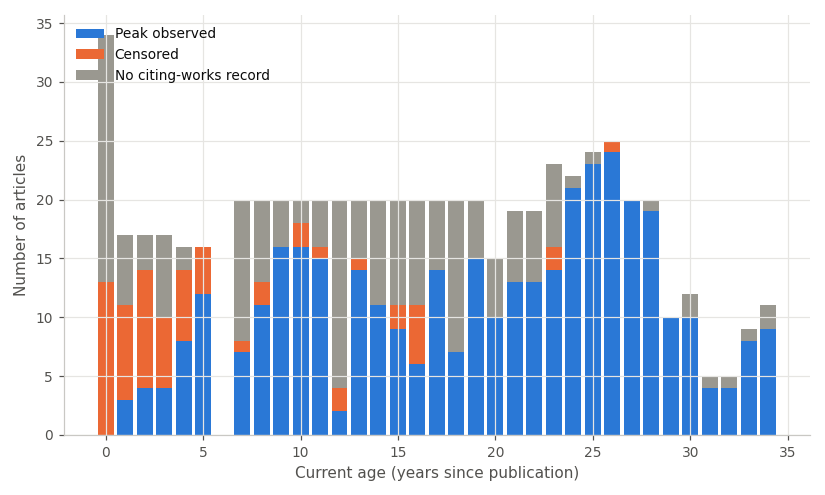
\includegraphics[width=0.65\textwidth]{figures/eda_censoring.png}
\end{figure}

Two features of the roster are worth noting alongside this. The dataset contains no FSR articles published in 2019, which appears as a break in the age profile. The 174 excluded articles are matching failures rather than uncited work: 114 of them carry Scopus citations, 909 in total. Entering them as censored observations would hold them in the risk set for their full age while never contributing an event, which raises the estimated median peak age from 7 years to 10.

Inspecting individual citation trajectories reinforces the case for a survival-analysis approach. Year-to-year citation counts for a given article are typically small and irregular rather than smooth, and many articles record several separate spikes across their lifetime rather than one clear rise and fall. A single observed maximum can therefore represent either a genuine peak or simply a stronger year, which is the ambiguity the censoring rule in Question D is designed to handle.

\begin{figure}[htbp]
\centering
\caption{Annual citation counts for individual articles are small and irregular, with many articles recording several separate spikes rather than a single clear peak.}
\label{fig:eda_trajectories}
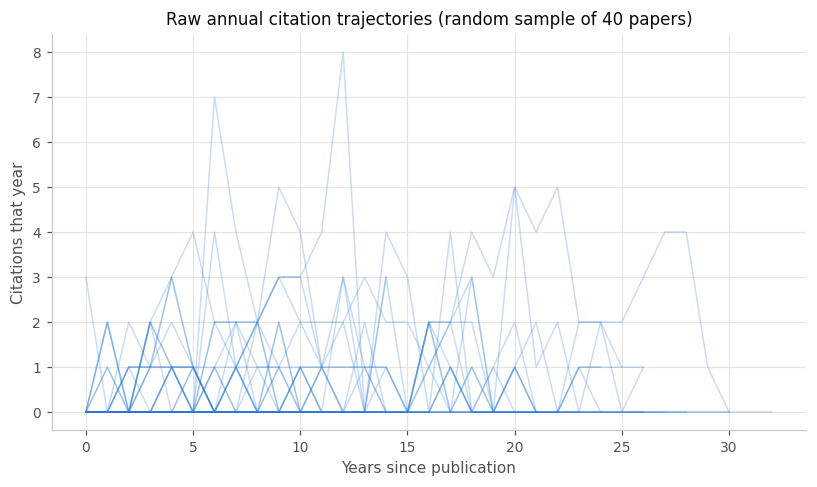
\includegraphics[width=0.65\textwidth]{figures/eda_trajectories.png}
\end{figure}

\subsubsection{Distribution of citations}\label{distribution-of-citations}

Citation counts across FSR are strongly right-skewed. The average article has 15.1 citations, but the median article has only 5, and the most cited article has 678. Around one in ten articles (59 articles, 10.1\%) have never been cited at all. Plotting the distribution on a logarithmic scale makes this clearer and shows that the 90th-percentile threshold used to define a high hitter in Question D (26 or more citations, 63 articles) sits well into the upper tail. This skew is also why the later modelling works with a top-decile threshold and log-transformed citation counts rather than raw averages.

\begin{figure}[htbp]
\centering
\caption{Citations are heavily right-skewed, with the high-hitter threshold of 26 citations sitting well into the upper tail.}
\label{fig:eda_distribution}
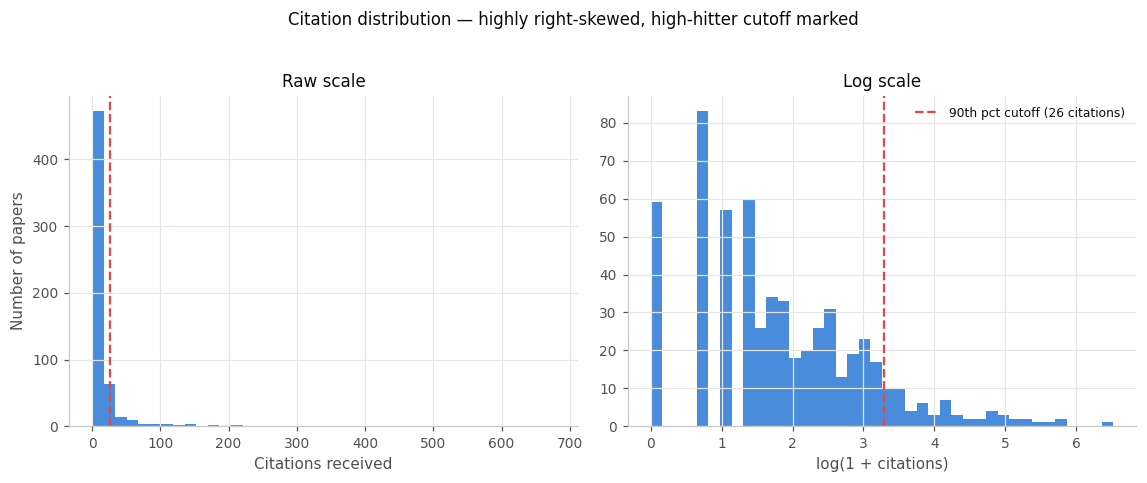
\includegraphics[width=0.75\textwidth]{figures/eda_citation_distribution.png}
\end{figure}

Citations are correspondingly concentrated in a small number of articles. The 582 articles collectively received 8,812 citations, but the top 10\% of articles account for close to two-thirds of that total, while the bottom half of articles account for 5.8\%.

\begin{table}[htbp]
\centering
\small
\caption{Concentration of citations across FSR articles (8,812 citations in total).}
\label{tab:eda_concentration}
\begin{tabular}{lrr}
\toprule
Group & Articles & Share of all citations \\
\midrule
Top 1\% of articles & 5 & 21.1\% \\
Top 10\% of articles & 58 & 63.7\% \\
Bottom 50\% of articles & 291 & 5.8\% \\
\bottomrule
\end{tabular}

\end{table}

\subsubsection{Article characteristics and their relationships}\label{article-characteristics-and-their-relationships}

The six bibliographic characteristics used in the Question D modelling are summarised below. Most FSR articles are produced by small author teams: two-author papers are the most common (45.2\%), followed by three-author papers (27.1\%) and single-author papers (20.8\%), with fewer than 7\% of articles having four or more authors. This limited spread is worth keeping in mind when interpreting the author-count result in Question D, because that association is estimated mainly from the difference between one-, two- and three-author papers.

\begin{table}[htbp]
\centering
\small
\caption{Descriptive statistics for the 582 FSR articles used in the high-hitter modelling.}
\label{tab:eda_descriptives}
\begin{tabular}{lrrrrr}
\toprule
Variable & Mean & SD & Median & Min & Max \\
\midrule
Citations received & 15.1 & 43.8 & 5 & 0 & 678 \\
Number of authors & 2.2 & 0.9 & 2 & 1 & 7 \\
Number of affiliations & 1.7 & 0.8 & 2 & 1 & 6 \\
Number of author keywords & 3.1 & 1.9 & 3 & 0 & 11 \\
Page length (pages) & 16.2 & 5.3 & 16 & 1 & 41 \\
Abstract length (words) & 122.7 & 38.1 & 113 & 3 & 453 \\
\bottomrule
\end{tabular}

\end{table}

Correlations among these six characteristics are mostly weak. The one moderate relationship is between the number of authors and the number of affiliations (r = 0.61), which is expected, since larger teams tend to span more institutions. Log-transformed article age, the form used in the modelling, is negatively related to page length (r = \(-0.40\)), keyword count (r = \(-0.34\)) and abstract length (r = \(-0.30\)), indicating that more recent FSR articles tend to be longer and more thoroughly indexed than older ones. No other pair exceeds 0.3. Even the author and affiliation pair remains within acceptable limits for modelling, with all variance inflation factors for the Question D model below 1.7, so the estimated associations can be read as largely independent rather than as artefacts of overlapping predictors.

\begin{figure}[htbp]
\centering
\caption{Author count and affiliation count are the only moderately related pair; the remaining characteristics carry largely independent information.}
\label{fig:eda_correlations}
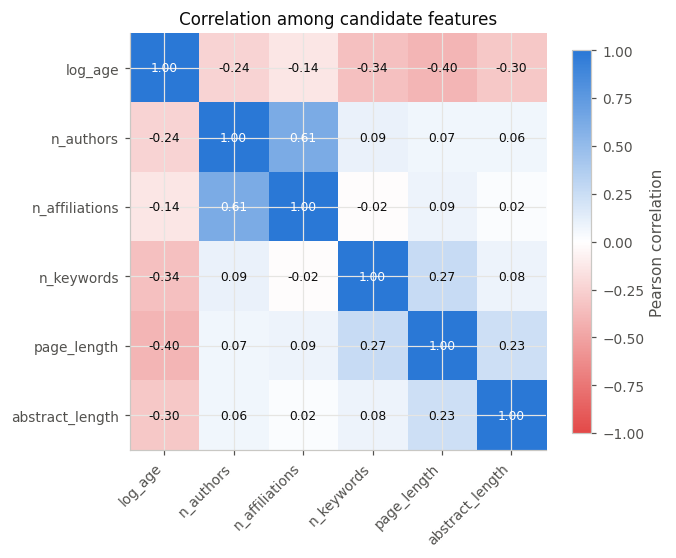
\includegraphics[width=0.55\textwidth]{figures/eda_correlations.png}
\end{figure}

\section{Methods and Design}\label{methods-and-design}

This section sets out the methods used to answer the four research questions.

\subsection{Do Star Authors Drive Citations? (Question A)}\label{do-star-authors-drive-citations-question-a}

The question was separated into three parts: whether FSR\textquotesingle s citations are concentrated among a small number of authors, whether the most-cited authors are the prolific ones or the well-known ones, and whether an author\textquotesingle s track record before an article appeared predicts how many citations that article has attracted. The analysis used the 1,360 attributable articles and 1,953 authors described in the Dataset section, together with the OpenAlex author records. Citations were whole-counted, so each co-author was credited with an article\textquotesingle s full citation count.

Concentration was measured within each journal by summing citations per author and computing the share held by the top 1\%, 5\% and 10\% of authors, the Gini coefficient and the Lorenz curve. The same statistics were computed across articles. This comparison matters because if a few articles hold most of the citations and most authors publish only once, author-level concentration follows arithmetically from article-level concentration whoever the authors are, and the two Gini coefficients will coincide. FSR was compared with FPR and JFCP throughout.

To test whether the most-cited authors are the prolific ones or the well-known ones, the 241 FSR authors with at least two FSR articles and an OpenAlex record were ranked three ways: by citations to their FSR articles, by number of FSR articles and by career h-index. Agreement between rankings was measured by Spearman rank correlation and by the number of names shared between the top 20 on each ranking.

Research topic was needed as a control so that an author's track record would not be credited for the subject they happen to work on. Rather than fit a separate model, Question A uses the final topic model from Question B: non-negative matrix factorisation (NMF) with eleven topics, fitted to the TF-IDF matrix of each article's combined title, abstract and author keywords (stop words and generic research terms removed, words lemmatised, unigrams to trigrams, minimum document frequency 5, maximum document frequency 85\%). Both questions therefore work from the same partition of the corpus. Each article was assigned to the topic with its largest weight, and every article received a topic. The eleven topics are listed in Appendix~\ref{app:topics}. This section uses shortened labels taken from each topic's top terms: retirement saving, credit card debt, portfolios and markets, household surveys, financial planning and advice, students and loans, and tax and withdrawals correspond to Appendix~\ref{app:topics}'s Retirement Planning, Credit and Debt, Portfolio Investment, Household Finance, Financial Advice, Student Finance and Tax and Retirement Accounts respectively. Question A uses portfolios and markets as the reference category because it is FSR's largest topic, whereas Question B uses Retirement Planning, so the two sets of topic coefficients are measured against different baselines and should not be compared directly.

The relationship between track record and citations was estimated with a negative binomial regression, since FSR citation counts are overdispersed (mean 14.2, variance 1,818). The sample was the 617 FSR articles with at least one OpenAlex-matched co-author; 8 of the 625 FSR articles were dropped. Three track-record measures were constructed for each article, each taken as the maximum over its matched co-authors: the number of works and the number of citations the author had accumulated in the years strictly before the article's publication year, taken from OpenAlex's year-by-year history so that nothing occurring after publication could leak into the predictor, and the author's current h-index. Because OpenAlex publishes only the present h-index, that measure includes reputation built after the article appeared and was treated as an upper bound; the model was therefore fitted both with h-index and prior citations together and with prior citations alone, the leak-free specification. Prior counts were log-transformed. The controls were log-transformed article age, number of authors and topic, with portfolios and markets, FSR's largest topic (166 articles), as the reference category. Variance inflation factors were checked before fitting; prior works were dropped (VIF 6.5, Spearman \(\rho\) = 0.88 with prior citations), after which every VIF was below 2.4. Because prior citations and h-index remain correlated (\(\rho\) = 0.85), a joint Wald test of the two terms was reported alongside the individual incidence rate ratios.

Predictive value was tested with a temporal holdout. The model was refitted on the 473 FSR articles published before 2018 and used to rank the 144 articles published from 2018 onward, which it had not seen, with performance measured by the Spearman correlation between predicted and actual citation counts. Four nested specifications (age and team size; adding track record; adding topic; adding both) separated the contribution of track record from that of topic. Two sensitivity checks were run. The main model was refitted without the 39 articles that have a co-author whose OpenAlex profile appears to merge several people (more than 300 works), and the same specification was fitted across all three journals with journal indicators. Journal two-year citedness could not be included in the pooled model because, with three journals, it is an exact linear combination of the journal indicators.

\subsection{Topic and Keyword Analysis~(Question B)}\label{topic-and-keyword-analysis-question-b}

For this analysis, we used topic modelling to identify the main research topics and keywords associated with citation performance and emerging trends in the personal financial planning field. Without prior evidence on which approach suits a corpus of 1,362 articles, we compared three: two traditional approaches based on document-term representations, Latent Dirichlet Allocation (LDA) and Non-negative Matrix Factorization (NMF), and BERTopic, which uses contextual embeddings to capture semantic relationships between terms.

LDA and NMF are well suited to a corpus of this size, but both rely on word co-occurrence rather than semantic meaning. As discussed previously, authors often describe the same concept in different terms (e.g., "financial literacy" vs.~"financial knowledge"). Models based on word co-occurrence treat such synonyms as unrelated, so they can split one theme across several topics. We included BERTopic to detect these semantic similarities, though it is typically applied to much larger datasets than the 1,362 articles analysed here.

For each article, we combined the title, abstract, and author keywords into a single text field to give a more complete textual representation. We then removed stopwords, applied lemmatisation to reduce words to their base form, and retained bigrams and trigrams to preserve meaningful domain-specific phrases (e.g., "risk tolerance" rather than "risk" and "tolerance"). Since all three journals focus on related areas, high-frequency domain and generic terms such as "research" or "study" were excluded from the analysis, as they contributed little to distinguish one topic from another.

For LDA and NMF, we selected a number of topics (k) using a coarse-to-fine search, with a final range of 6 to 11, and computed \(C_{v}\) coherence for each k. LDA was fitted to a document-term count matrix using batch learning, while NMF was fitted to a TF-IDF matrix. For both models, we excluded terms appearing in fewer than five articles or in more than 90\% of articles. Using the same coarse-to-fine approach, we tuned the minimum number of documents per topic (min\_topic\_size) for BERTopic, which derives the number of topics from HDBSCAN clustering, with a final range of 23 to 25. We transformed each article's combined text into embeddings, reduced them with UMAP and clustered them with HDBSCAN. We then reassigned articles initially classified as outliers (-1) to their closest topic using c-TF-IDF similarity.

We evaluated LDA and NMF using \(C_{v}\) coherence score as the primary metric, calculated from each topic\textquotesingle s top 10 words. It measures how semantically related a topic's top words are, based on how often they co-occur in the corpus (Röder et al., 2015). We also computed perplexity for LDA as a secondary metric, where lower values indicate a better statistical fit. When selecting the final model, we prioritised coherence and topic interpretability over perplexity, as the analysis focuses on meaningful themes, not maximising statistical fit (Wang \& Aryani, 2025). Similarly, we evaluated BERTopic by checking whether the top-ranked terms in each topic formed a meaningful theme.

After selecting the final model, we fitted a negative binomial regression of citation counts on article-level topic proportions, controlling for log-transformed paper age and journal:

\[\log(\mu_i) = \beta_0 + \sum_k \beta_k\, p_{ik} + \gamma \log(\text{age}_i) + \sum_j \delta_j\, \text{journal}_{ij}\]

where \(\mu_i\) is the expected citation count for article \(i\), \(\text{age}_i\) is its age in years, \(p_{ik}\) is the proportion of its text assigned to topic \(k\), and \(\text{journal}_{ij}\) are journal indicators. Since citations accumulate over time, older articles have greater citation exposure than more recently published papers, so we included article age as a control variable in the regression model. To further account for differences in citation accumulation over time, article age was log-transformed, as citation growth tends to slow as articles become older. To compare high- and low-cited articles, we ranked articles by citations per year within each journal and compared mean topic proportions between the highest and lowest quartiles.

\subsection{Abstract Readability and Citation Counts (Question C)}\label{abstract-readability-and-citation-counts-question-c}

The brief asks whether a clearly written abstract attracts more citations. An abstract is one of the few things an editor can ask an author to change before publication, so the practical value of the question depends on whether any association is strong enough, and specific enough to FSR, to justify that request. We therefore answered it in two stages: first whether readability is associated with citations at all, then whether that association is the same in FSR as in the comparator journals.

Readability was measured with the Gunning Fog Index as the primary scale, with the Flesch Reading Ease and Flesch-Kincaid Grade Level as alternatives. All three combine sentence length with a word-difficulty term, but they weight those components differently: Fog counts words of three or more syllables, while the two Flesch measures use syllables per word. Reporting all three guards against a result that depends on one formula's particular weighting, and the Flesch Reading Ease runs in the opposite direction to the other two, so a genuine association should appear as a sign reversal rather than as agreement. Scores were computed with the \texttt{textstat} package. Before scoring, abstracts were stripped of copyright statements, which are boilerplate rather than author prose and would otherwise inflate sentence length for the journals that append them.

The sample is the 1,353 articles with a usable abstract and an author list. Seven records carry the placeholder ``[No abstract available]'' and have no text to score, and two have no author identifier.

Citation counts are overdispersed, so citation-count models use negative binomial regression throughout (see the modelling approach). Paper age enters as \(\log(2026 - \text{year} + 1)\), the same form Question A uses, which counts years from publication to the end of the extraction year and keeps a defined logarithm for articles published in 2026. Question D measures age to 2025 instead, because its outcome is the OpenAlex citation trajectory, which ends at the last complete year, whereas here the outcome is the cumulative Scopus count at extraction, so exposure runs to 2026. The log form is used rather than a linear one because citation accrual decelerates, and it gave the lower AIC. Number of authors is included because Question D finds team size associated with citations, and larger teams could plausibly write differently.

Age is the central confound rather than an incidental control. Fog scores are negatively correlated with age in every journal (\(\rho\) = \(-0.26\) in FSR, \(-0.33\) in JFCP and \(-0.21\) in FPR), so older articles are both more readable and, having been available longer, more cited. Any unadjusted comparison therefore pushes the readability-citation association towards zero, which is what the raw correlations show. This is why the adjusted and unadjusted results point in opposite directions, and why the adjusted estimate is the one to read.

A pooled model with journal indicators was the starting point, but it constrains every journal to share one readability slope and so cannot answer whether FSR behaves like its comparators. Because the project's question is about FSR specifically, the analysis was extended in two ways. First, the model was refitted separately within each journal, which lets the slope differ without imposing any structure on how. Second, a readability-by-journal interaction was fitted on the pooled data and compared with the no-interaction model by likelihood-ratio test, which asks directly whether one slope is enough. The stratified fits show the size and direction of any difference; the interaction test says whether the difference is larger than sampling noise. Reporting only one of the two would leave either the magnitude or its reliability unstated.

Two further controls were added as sensitivity checks. Abstract length is correlated with both readability and citations and could drive any association on its own, so it enters as a covariate. Research topic was added using the eleven-topic model selected under Question B, the same partition Questions A and D use, because technical subfields may be both harder to read and differently cited, and without that control a topic effect could be mistaken for a readability effect.

\subsection{Citation Trajectories and High Hitters (Question D)}\label{citation-trajectories-and-high-hitters-question-d}

The brief asks when FSR papers peak and whether the eventual high performers can be spotted early. These are two different decisions for AFS, so we answered them separately. Timing determines how long the journal should wait before judging a paper at all; predictability determines whether the bibliographic record is informative enough to judge it in advance. Part 1 used Kaplan--Meier survival analysis, Part 2 logistic regression with quantile regression as a supporting check.

Part 1 needed a method from outside the literature reviewed earlier, which models how many citations an article receives rather than when they arrive. The direct approach, averaging each paper's highest-citation year, assumes every observed maximum is final: a paper published in 2022 has only three complete years of history by 2025, so its maximum is confined to those years regardless of whether citations are still climbing, pulling the average down for exactly the cohort AFS cares most about. Treating the peak as a right-censored event removes that bias, recording a still-rising paper as not yet peaked rather than forcing an artificial peak on it. Kaplan--Meier was chosen over a parametric alternative because the question is descriptive: a Weibull model would impose a hazard shape no theory of citation behaviour supports, and a Cox model estimates how covariates shift the hazard, which is Part 2's question. The resulting estimand is the time to an \textit{observed} peak within the available window, not proof that no later year could exceed it, and results are reported on those terms throughout.

Scopus supplies one cumulative citation count per article and no year-by-year history, so Part 1 required reconstructing an annual citation trajectory for every FSR article from OpenAlex's citing works, aggregated by publication year (see Dataset). The 174 papers with no citing-works record were excluded rather than entered as censored, for the reasons set out there; this left the 442 papers analysed below. That exclusion is not spread evenly across publication era: 6.8\% of 1990s papers were excluded for lacking an OpenAlex match, against 29.2\% of 2000s papers and 36.0\% of papers from 2010 onward (\(\chi^2\) = 35.4, \(p < .001\)), consistent with OpenAlex indexing lag rather than citation behaviour. The most recent era bucket in the landmark comparison below is therefore drawn from the least complete subsample of the three, and its results should be read with that in mind. The Kaplan--Meier estimator gives the probability that a paper has not yet reached its citation peak by age $t$:

\[\hat{S}(t) = \prod_{t_{(j)} \le t} \left(1 - \frac{d_j}{n_j}\right)\]

where \(n_j\) is the number of papers still ``at risk'' of peaking just before age \(t_{(j)}\), and \(d_j\) is the number that peak exactly at that age.

To test whether peak timing has changed over the journal's history, a separate curve was fitted for three publication eras, split by calendar decade (1990s, 2000s, 2010s onward) rather than chosen after inspecting the curves, and compared with a log-rank test, the non-parametric companion to Kaplan--Meier. That comparison is informative only if the three eras are observed on equal terms, and over their full available histories they are not: a paper published in 1995 can be seen peaking at age 25, while a 2018 paper is observed for only seven years and cannot record a late peak at all, so the test rewards whichever cohort has been watched longest. Run that way it returns median peak ages of 10, 7 and 4 years at $p < .001$, which would read as a steady three-decade acceleration. We therefore added a landmark analysis, observing every paper over the same ages 0 to $H$ and including only papers old enough to complete that window, so an observed peak carries the same meaning in each era. A horizon of eight years leaves all three eras with at least 104 articles while still allowing a full window for a peak to appear. Pairwise log-rank tests are reported alongside the overall test, since an overall test can reach significance on one contrast while the contrast of interest is null.

Part 2 needs a different outcome. The exploratory analysis shows the top 10\% of FSR papers holding 63.7\% of the journal's citations while the bottom half contribute 5.8\%, so the editorially useful question is not what moves a typical paper by a few citations but what separates the small group that carries the journal. We therefore defined a high hitter on the upper tail, as a paper at or above the 90th percentile of citation counts (\(\geq 26\) citations in this sample), giving 63 of 582 modelled papers (10.8\%) rather than exactly 10\% because several papers sit on the cutoff.

Three alternatives were considered for modelling that outcome. Linear regression on raw counts was rejected because citations are strongly right-skewed, which breaches its assumptions and permits negative predictions. Poisson regression was rejected because it assumes the variance equals the mean, and in this sample the variance is roughly 127 times the mean. Negative binomial regression accommodates that overdispersion and is the family Didegah and Thelwall (2013) build their hurdle model on, but it describes the conditional mean, and where a handful of papers dominate the distribution the mean is not the quantity AFS acts on. We used logistic regression because it estimates the probability that a given paper clears the threshold that matters, as a function of six bibliographic features: log-transformed paper age, number of authors, number of affiliations, number of author keywords, page length and abstract length:

\[\operatorname{logit}(p_i) = \ln\frac{p_i}{1 - p_i} = \beta_0 + \beta_1\,\text{log\_age} + \beta_2\,\text{n\_authors} + \dots + \beta_6\,\text{abstract\_length}\]

Each coefficient converts to an odds ratio, \(\text{OR} = e^{\beta}\), which describes how the odds of being a high hitter change for a one-unit increase in that characteristic, holding the others constant.

The six characteristics adapt the document-characteristics block used by Didegah and Thelwall (2013). Our addition is a selection criterion they do not apply: a characteristic was admitted only if an editor could observe it at the point of an editorial decision, since a variable that becomes knowable only years later cannot inform that decision however well it correlates with citations. That criterion is what excludes journal impact factor, the strongest single predictor in their study, because it is constant within a single journal and so cannot inform any choice AFS is in a position to make. Within that constraint, number of authors captures collaboration, the characteristic most consistently linked to citation performance across the studies reviewed; number of affiliations captures institutional spread, as a proxy for how many research networks a paper reaches; number of author keywords captures indexing breadth, and so how discoverable a paper is through database search; page length stands for the scope of the work; and abstract length for how much of the paper a reader sees when deciding whether to read on. Log-transformed paper age enters as an exposure control rather than a characteristic of interest, because older papers have simply had longer to accumulate citations, and the log form reflects that citation accrual decelerates with time.

Several further characteristics were considered and left out, for reasons ranging from zero variance to data availability to keeping Part 2 a clean test of the structural record on its own; Appendix~\ref{app:qd_excluded} lists each and why. Number of authors and number of affiliations are correlated at $r = 0.61$, because the affiliation field records one entry per author, but both were retained because every variance inflation factor was below 1.7 and neither variable is redundant by that test.

Before interpreting the coefficients, four diagnostics were run, each addressing a specific way a logistic model can mislead. The Box--Tidwell test checks whether each continuous predictor is linear on the log-odds scale, which the model assumes. Variance inflation factors check whether predictors are collinear enough to destabilise individual coefficients. Cook's distance screens for single papers influential enough to drive the fit alone, which is a live risk where a few articles hold most of the citations. Events per variable checks whether the positive class supports six predictors, since for a rare outcome the usable sample size is the number of events rather than the number of papers; with 63 events and six predictors the ratio is 10.5, only marginally above the conventional threshold, so we treat findings near $p = .05$ as suggestive rather than settled.

Three further checks were run on the fitted model. Because an odds ratio is defined on a binary outcome, it is not directly comparable with the incidence rate ratios reported for Questions A and C, so we refitted the same specification as a negative binomial regression on the citation count, which places all three questions on one scale. The model was then refitted with individual controls removed, to establish whether the reported associations depend on one particular combination of predictors. Finally, research topic was added as a control in both the logistic and count-scale models, because topic is the strongest driver of citations identified in this project and omitting it risks crediting other characteristics with its effect. Rather than fit a separate topic model, we used the eleven-topic NMF model selected under Question B, the same partition Question A uses, so that the three questions work from one set of topic definitions.

The logistic regression answers whether a paper clears the high-hitter threshold, but in doing so it reduces citation performance to a yes or no outcome. This creates two limitations. First, it discards information about magnitude, treating a paper with 26 citations and a paper with 678 as equivalent outcomes. Second, the 90th-percentile threshold is a modelling choice rather than a property of the data, and a result that depended on that particular cutoff would be difficult to rely on. Quantile regression addresses both: it estimates the relationship separately at chosen points of the citation distribution and requires no threshold at all, which suits data as skewed as FSR's, and because the estimates are anchored to quantiles rather than to a mean they are not distorted by the small number of very highly cited articles. The coefficients at quantile \(\tau\) are obtained by minimising asymmetrically weighted absolute errors:

\[\hat{\beta}(\tau) = \arg\min_{\beta} \sum_i \rho_\tau\!\left(y_i - x_i^{\top}\beta\right), \qquad \rho_\tau(u) = u\left(\tau - \mathbf{1}\{u < 0\}\right)\]

where the outcome \(y_i\) is \(\log(1 + \text{citations})\) and the model is estimated at \(\tau\) = 0.10, 0.25, 0.50, 0.75 and 0.90. Comparing coefficients across these points shows whether a characteristic behaves consistently across the journal or matters mainly at the top of the distribution, which is the part of most interest to AFS given how concentrated citations are. Sienkiewicz and Altmann (2016) used quantile regression for the same reason and reported that several article characteristics behaved differently among highly cited papers than among papers with more typical counts. They read that pattern from the coefficient path rather than testing it, so we tested the difference between the coefficient at \(\tau\) = 0.90 and the coefficient at \(\tau\) = 0.50 directly, by resampling papers with replacement over 600 bootstrap replicates, and refitted the logistic model at thresholds corresponding to the top 50\%, 25\%, 10\% and 5\% of papers, which puts the same question on a single consistent scale and shows whether any tail effect is monotone rather than an artefact of one cutoff.

\section{Results}\label{results}

\subsection{Question A: Do Star Authors Drive Citations?}\label{question-a-do-star-authors-drive-citations}

Citations are concentrated in every journal (Table~\ref{tab:qa_conc}). In FSR the top 1\% of authors (10 people) hold 24.3\% of all citations to the journal, the top 5\% hold 52.3\% and the top 10\% hold 66.3\%, with a Gini coefficient of 0.762. JFCP\textquotesingle s figures are the same to within a percentage point, and FPR, a younger and smaller journal, is slightly less concentrated. Concentration across FSR articles is almost identical to concentration across FSR authors (Gini 0.755 against 0.762), and 75.1\% of FSR authors have published in the journal exactly once, so for most of the author base an author\textquotesingle s citation total is one article\textquotesingle s citation count relabelled (Figure~\ref{fig:qa_relabel}). JFCP is the exception: its article-level Gini (0.676) sits well below its author-level Gini (0.765), which is the signature of a group of returning authors who concentrate citations beyond what the article distribution implies. Individual JFCP authors have contributed up to 36 articles, against a maximum of 14 in FSR.

\begin{table}[htbp]
\centering
\small
\caption{Citation Concentration by Journal}
\label{tab:qa_conc}
\begin{tabular}{lrrrrrrr}
\toprule
Journal & Authors & Top 1\% & Top 5\% & Top 10\% & \makecell[r]{Gini\\(authors)} & \makecell[r]{Gini\\(articles)} & \makecell[r]{One-time\\authors (\%)} \\
\midrule
FSR & 966 & 24.3\% & 52.3\% & 66.3\% & 0.762 & 0.755 & 75.1 \\
FPR & 203 & 17.2\% & 43.5\% & 60.2\% & 0.735 & 0.759 & 76.8 \\
JFCP & 1,006 & 25.0\% & 53.3\% & 66.0\% & 0.765 & 0.676 & 77.1 \\
\bottomrule
\end{tabular}
\tablenote{Top 1\%, 5\% and 10\% are the shares of the journal's citations held by its most-cited authors under full counting. One-time authors are those with a single article in the journal.}
\end{table}

\begin{figure}[htbp]
\centering
\caption{Article-Level and Author-Level Citation Inequality by Journal}
\label{fig:qa_relabel}
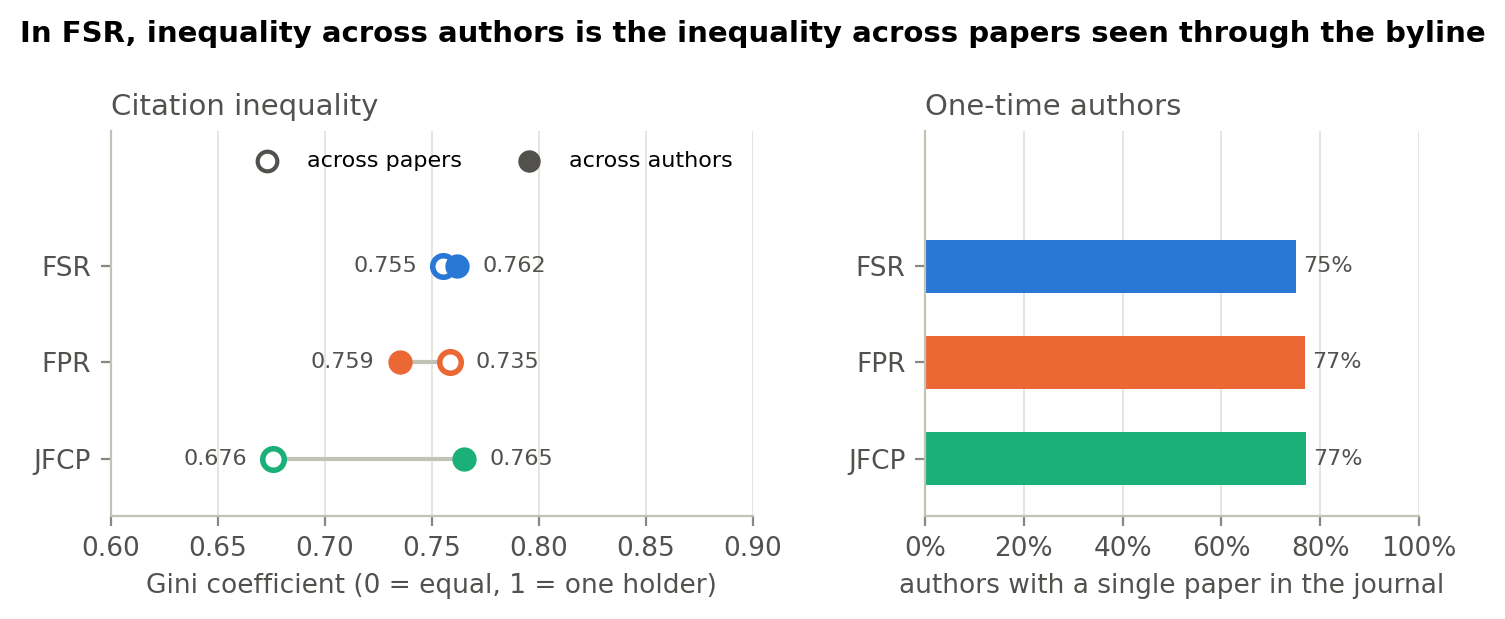
\includegraphics[width=0.95\textwidth]{figures/qa_paper_vs_author.png}
\end{figure}

The most-cited FSR authors are not, in general, the most prolific or the best known (Table~\ref{tab:qa_top}). Haiyang Chen and Ronald P. Volpe, who co-wrote the two most-cited articles in the journal\textquotesingle s history, tie at the top with 1,074 citations from three FSR articles each, and several of the ten have a career h-index below 10. Among the 241 repeat FSR authors, the rank correlation between FSR citations and FSR article count is 0.41, between FSR citations and career h-index 0.30, and between article count and h-index 0.27. The three top-20 lists share few names: 6 authors appear on both the most-cited and most-prolific lists, 5 on the most-cited and highest-h-index lists, and 3 on the most-prolific and highest-h-index lists (Figure~\ref{fig:qa_three}).

\begin{table}[htbp]
\centering
\small
\caption{The Ten Most-Cited FSR Authors}
\label{tab:qa_top}
\begin{tabular}{lrrr}
\toprule
Author & FSR articles & Citations to FSR articles & Career h-index \\
\midrule
Haiyang Chen & 3 & 1,074 & 24 \\
Ronald P. Volpe & 3 & 1,074 & 5 \\
John E. Grable & 10 & 531 & 44 \\
Ruth H. Lytton & 3 & 458 & 8 \\
Robert W. Faff & 2 & 293 & n/a$^{*}$ \\
Sherman D. Hanna & 14 & 291 & 30 \\
Terrence Hallahan & 1 & 279 & 10 \\
Michael D. McKenzie & 1 & 279 & 30 \\
H. Kent Baker & 6 & 275 & 50 \\
Catherine P. Montalto & 6 & 252 & 22 \\
\bottomrule
\end{tabular}
\tablenote{h-index is the OpenAlex value at September 2026. $^{*}$Matched to a fragmentary OpenAlex profile (one work, no citations); the real value is far higher.}
\end{table}

\begin{figure}[htbp]
\centering
\caption{FSR Citations Against Output and Reputation for Repeat FSR Authors}
\label{fig:qa_three}
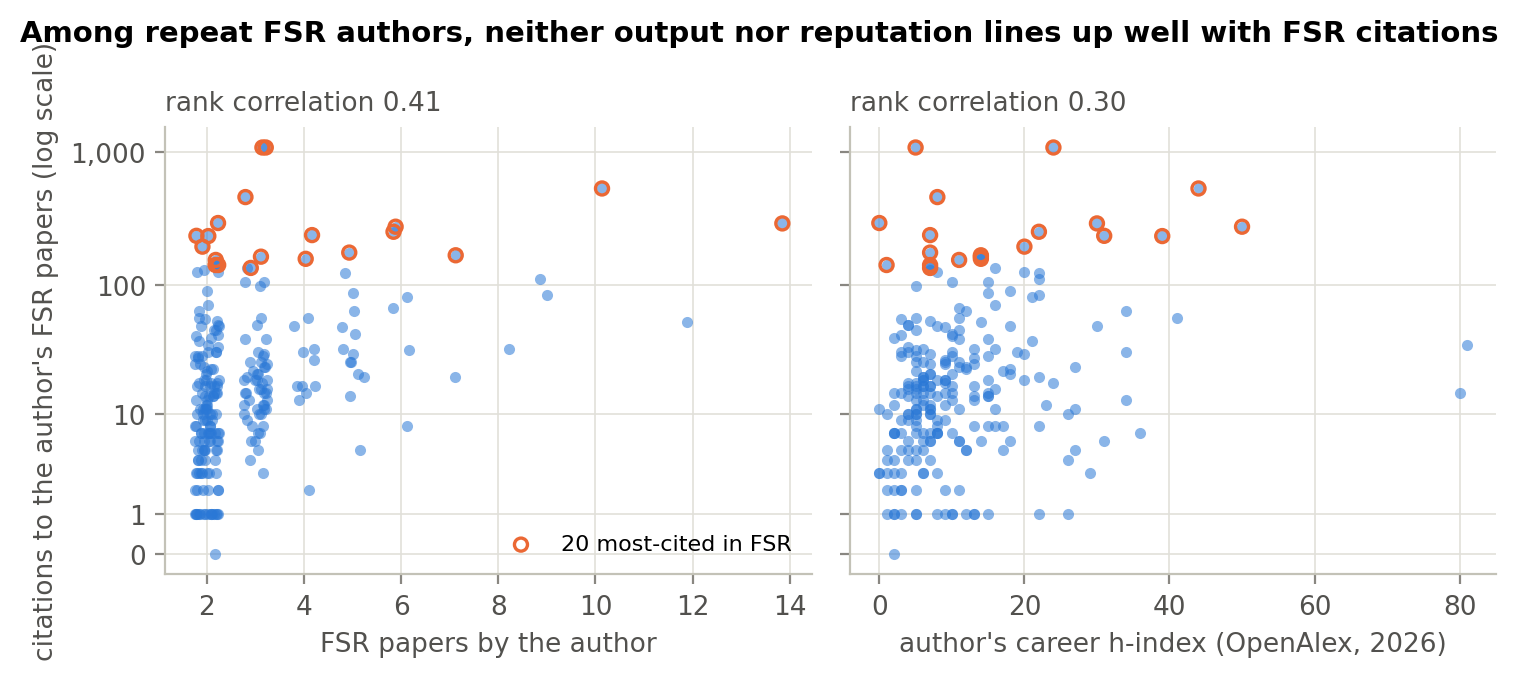
\includegraphics[width=0.95\textwidth]{figures/qa_prolific_vs_wellknown.png}
\end{figure}

Topic explains much of where FSR's citations come from (Figure~\ref{fig:qa_topic}). FSR's most-cited topics are risk tolerance (2.4 citations per article per year, 30 articles) and financial literacy (2.1, 35 articles), followed by students and loans (1.4, 35 articles) and financial behaviour (1.1, 35 articles). Its largest topic, portfolios and markets (166 articles), and the related topics of mutual funds (74), tax and withdrawals (63) and retirement saving (45) together make up 56\% of FSR's articles, and each draws 0.5 citations per article per year or fewer. JFCP's mix runs the other way: it publishes six times as many financial behaviour articles as FSR (214 against 35) and more on household surveys (137 against 58), students and loans (59 against 35) and financial literacy (46 against 35), but only 19 on portfolios and markets. The students and loans figure rests partly on Chen and Volpe's 1998 and 2002 studies of financial literacy among college students, the two most-cited articles in FSR, which the topic model places there because their vocabulary centres on students. Repeat FSR authors follow the same skew: 60 of the 241 work mainly on portfolios and markets and 130 (54\%) on one of the four investment, retirement and tax topics, and a repeat author's dominant topic covers 60\% of their articles on average.

\begin{figure}[htbp]
\centering
\caption{FSR Citation Rate by Topic and Topic Mix Against JFCP}
\label{fig:qa_topic}
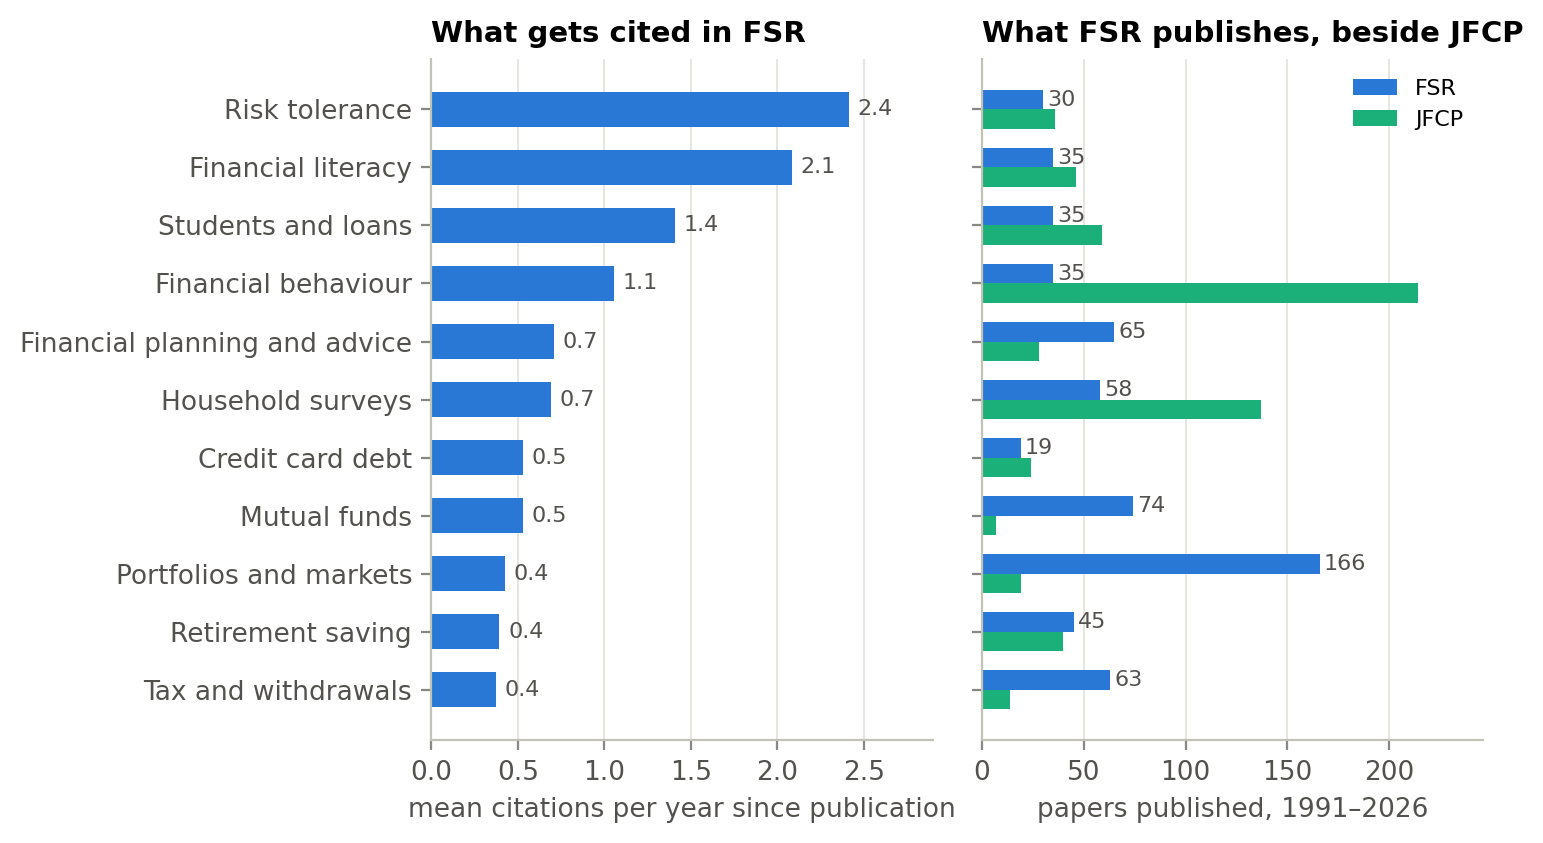
\includegraphics[width=0.95\textwidth]{figures/qa_topic_mix.png}
\end{figure}

Table~\ref{tab:qa_model} and Figure~\ref{fig:qa_effects} report the negative binomial model. The two track-record terms are jointly significant (Wald \(\chi^2(2)\) = 25.3, p \textless{} .001) but individually small. With both in the model, h-index carries the effect (IRR = 1.016 per point, 95\% CI: 1.006--1.027, p = .001), so an article whose best-established co-author has an h-index 10 points higher is expected to attract 1.18 times the citations (95\% CI: 1.06--1.30), and prior citations add nothing further (IRR = 1.024, p = .509). In the leak-free specification without h-index, prior citations are significant on their own (IRR = 1.110 per log unit, 95\% CI: 1.057--1.167, p \textless{} .001), which corresponds to 1.08 times the citations (1.04--1.11) for each doubling of the best co-author's prior citation count. The controls are larger. Doubling article age multiplies expected citations by 2.59, and relative to a portfolios and markets article of the same age, team size and authorship, a financial literacy article is expected to attract 7.12 times the citations (95\% CI: 4.51--11.26), a risk tolerance article 4.72 times (2.94--7.59), a financial behaviour article 3.48 times (2.13--5.68) and a students and loans article 3.30 times (2.13--5.12). Financial planning and advice (1.95) and household surveys (1.72) also sit above the reference. Mutual funds (IRR = 1.28, p = .156), retirement saving (0.98, p = .908), tax and withdrawals (0.87, p = .444) and credit card debt (1.21, p = .559) are not distinguishable from portfolios and markets, and the number of co-authors has no detectable effect (IRR = 1.062, p = .318). The model's McFadden pseudo R\textsuperscript{2} is 0.082, so the fitted model accounts for little of the variation in FSR citation counts.

\begin{table}[htbp]
\centering
\small
\caption{Negative Binomial Model of FSR Article Citations (n = 617)}
\label{tab:qa_model}
\begin{tabular}{lrrr}
\toprule
Predictor & IRR & 95\% CI & p-value \\
\midrule
Best co-author's h-index (per point) & 1.016 & 1.006--1.027 & .001 \\
Best co-author's prior citations (log) & 1.024 & 0.955--1.098 & .509 \\
Prior citations (log), model without h-index & 1.110 & 1.057--1.167 & $<$ .001 \\
Article age (log) & 3.942 & 3.365--4.618 & $<$ .001 \\
Number of authors & 1.062 & 0.944--1.195 & .318 \\
Topic: financial literacy & 7.125 & 4.507--11.262 & $<$ .001 \\
Topic: risk tolerance & 4.724 & 2.941--7.588 & $<$ .001 \\
Topic: financial behaviour & 3.479 & 2.131--5.677 & $<$ .001 \\
Topic: students and loans & 3.300 & 2.128--5.119 & $<$ .001 \\
Topic: financial planning and advice & 1.948 & 1.340--2.832 & $<$ .001 \\
Topic: household surveys & 1.716 & 1.175--2.507 & .005 \\
Topic: mutual funds & 1.279 & 0.910--1.799 & .156 \\
Topic: credit card debt & 1.206 & 0.643--2.260 & .559 \\
Topic: retirement saving & 0.976 & 0.645--1.476 & .908 \\
Topic: tax and withdrawals & 0.869 & 0.606--1.246 & .444 \\
\bottomrule
\end{tabular}
\tablenote{IRR = incidence rate ratio; CI = confidence interval. Topic effects are relative to portfolios and markets, FSR's largest topic. Track-record measures are the maximum over the article's OpenAlex-matched co-authors. Joint Wald test of h-index and prior citations: $\chi^2(2)$ = 25.3, p $<$ .001. Pseudo R\textsuperscript{2} = 0.082 (0.079 in the model without h-index).}
\end{table}

\begin{figure}[htbp]
\centering
\caption{Estimated Multipliers on Expected Citations From the Negative Binomial Model}
\label{fig:qa_effects}
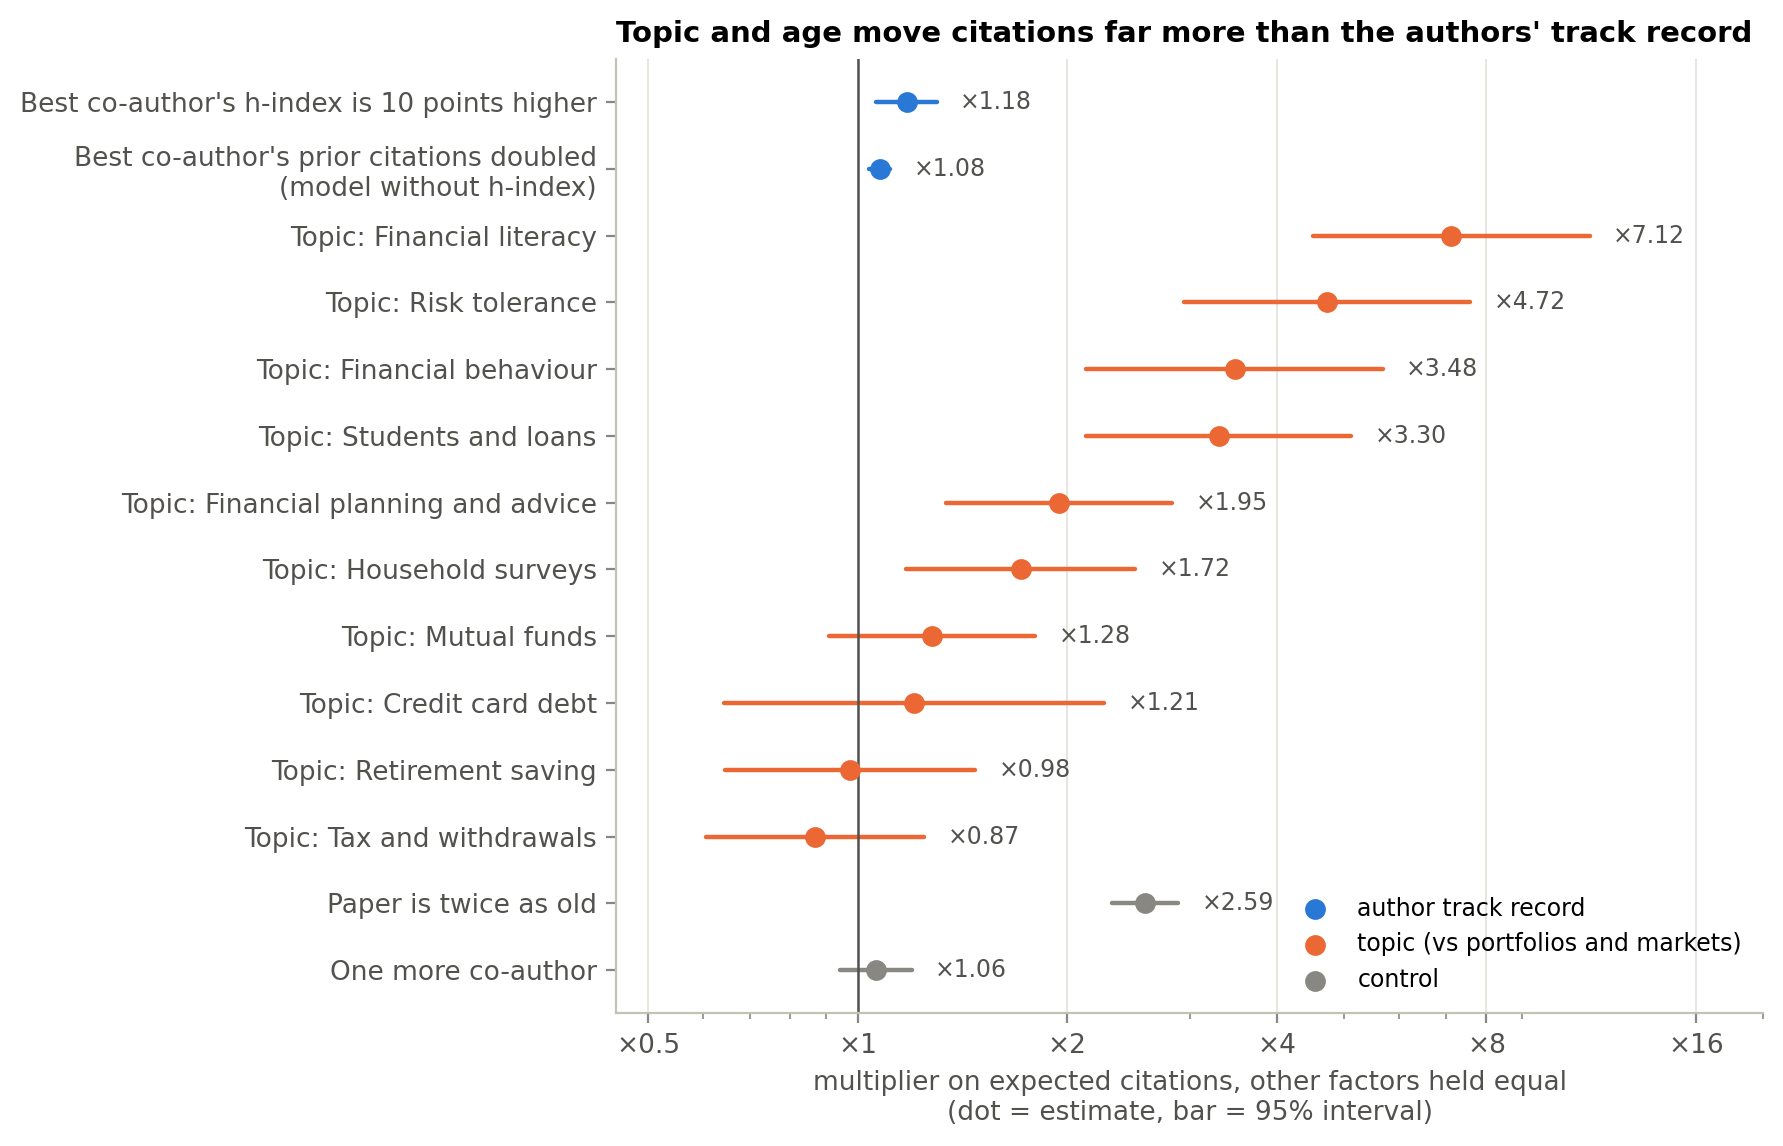
\includegraphics[width=0.85\textwidth]{figures/qa_model_effects.png}
\end{figure}

Out of sample, track record helps a little. Fitted on FSR articles published before 2018, a model with only article age and team size ranks the 144 unseen articles from 2018 onward with a Spearman correlation of 0.256 against their actual citations. Adding track record lifts this to 0.298, adding topic instead gives 0.285, and adding both gives 0.324. Removing the 39 articles with a suspect OpenAlex profile shifts weight between the h-index and prior-citation terms (IRR 1.027 and 0.994 respectively), as expected for two collinear measures, but leaves their combined effect and every control essentially unchanged. In the pooled model across all three journals (n = 1,317), prior citations remain significant (IRR = 1.124, 95\% CI: 1.076--1.174) and, with age, team size, topic and track record held constant, an article in JFCP is expected to attract 1.69 times the citations of the same article in FSR (95\% CI: 1.43--1.99) and an article in FPR 2.02 times (1.51--2.71).

\subsection{Question B: Which Topics Attract Citations, and Where Is FSR Thin?}\label{question-b-which-topics-attract-citations}

\subsubsection{Model comparison}\label{qb-model-comparison}

LDA performed best at \(k\) = 6--7, with a \(C_v\) coherence of 0.723, while NMF reached its maximum at \(k\) = 4 with 0.741. LDA perplexity fell steadily as \(k\) increased, from 1306.78 at \(k\) = 4 to a minimum of 1182.55 at \(k\) = 11, so coherence and perplexity did not agree on a single optimum for LDA.

\begin{table}[htbp]
\centering
\small
\caption{Coherence and perplexity by number of topics (k), LDA and NMF}
\label{tab:qb_k}
\begin{tabular}{rrrr}
\toprule
$k$ & LDA coherence & LDA perplexity & NMF coherence \\
\midrule
4 & 0.713 & 1306.78 & 0.741 \\
5 & 0.638 & 1308.94 & 0.722 \\
6 & 0.723 & 1251.69 & 0.700 \\
7 & 0.722 & 1250.34 & 0.695 \\
8 & 0.704 & 1236.27 & 0.705 \\
9 & 0.691 & 1205.34 & 0.715 \\
10 & 0.666 & 1187.21 & 0.711 \\
11 & 0.677 & 1182.55 & 0.707 \\
12 & 0.691 & 1186.97 & 0.671 \\
\bottomrule
\end{tabular}
\tablenote{Coherence is $C_v$, calculated from each topic's top 10 words; higher values indicate more interpretable topics. Perplexity is computed on the training corpus; lower values indicate a better statistical fit.}
\end{table}

\begin{figure}[htbp]
\centering
\caption{Coherence and perplexity across candidate topic counts for LDA and NMF.}
\label{fig:qb_coherence}
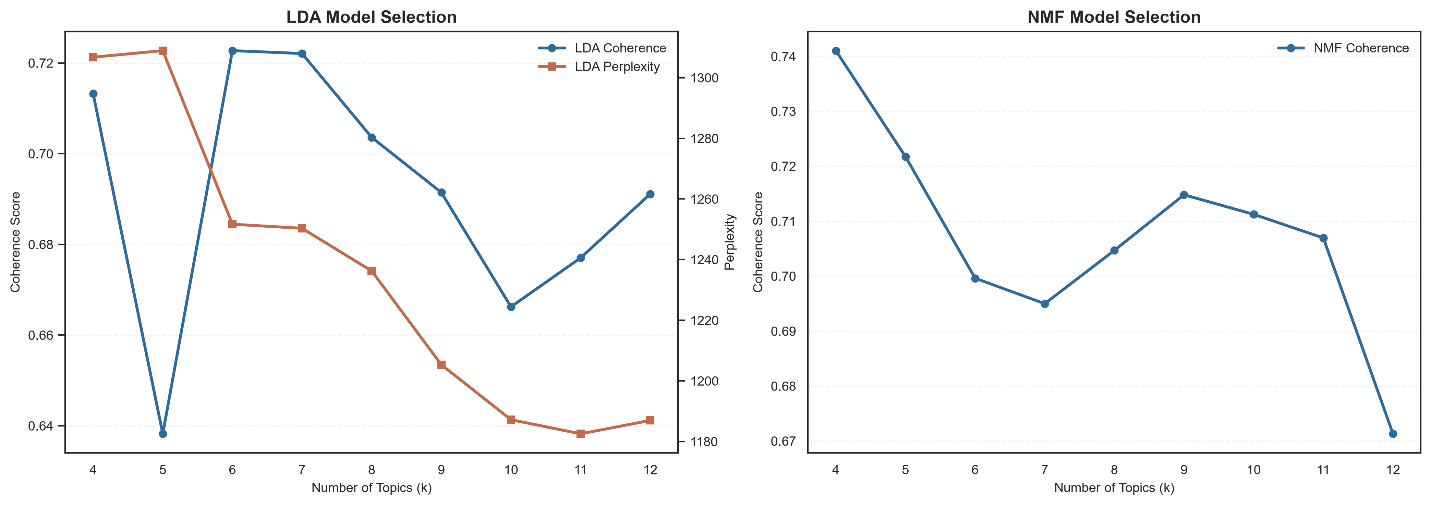
\includegraphics[width=\textwidth]{figures/qb_coherence.png}
\end{figure}

Although NMF at \(k\) = 4 scored highest on coherence, the resulting topics were broad and mixed several concepts together: financial literacy and student finance shared one topic at \(k\) = 4 before separating at higher \(k\). The coherence-maximising solution was therefore not the most useful one, and we also judged higher-\(k\) models on the distinctiveness of their top terms and whether each topic represented a single theme.

For BERTopic, coherence rose from 0.687 to 0.752 above a minimum topic size of 26, but that reflected the model collapsing to two topics, one holding most of the corpus, rather than a real improvement. Within the stable range, coherence peaked at a minimum topic size of 24--25 (\(\approx\) 0.688), giving a 15-topic solution.

\begin{table}[htbp]
\centering
\small
\caption{BERTopic model selection across minimum topic size}
\label{tab:qb_bertopic}
\begin{tabular}{rrrrr}
\toprule
min\_topic\_size & Topics & Outlier ratio (\%) & Topic size SD & Coherence \\
\midrule
20 & 18 & 40.82 & 25.14 & 0.665 \\
21 & 16 & 37.44 & 40.67 & 0.662 \\
22 & 13 & 26.28 & 87.33 & 0.627 \\
23 & 14 & 34.88 & 44.13 & 0.666 \\
24 & 15 & 37.67 & 34.99 & 0.688 \\
25 & 15 & 39.06 & 32.98 & 0.680 \\
26 & 14 & 41.92 & 29.99 & 0.687 \\
27 & 2 & 3.16 & 877.52 & 0.752 \\
\bottomrule
\end{tabular}
\tablenote{Outlier ratio is the share of articles left unassigned before c-TF-IDF reassignment.}
\end{table}

BERTopic surfaced several themes the bag-of-words models did not separate on their own: race and ethnicity in financial behaviour, COVID-19-related financial stress, and financial socialisation of families and young adults. Against that, it left 37.7\% of articles unassigned at its best-performing setting, where LDA and NMF classify every article by construction. Given a corpus of 1,362 articles and BERTopic's reliance on much larger datasets for stable clustering, we selected NMF with \(k\) = 11 as the final model, which gave complete and interpretable topic assignment at competitive coherence. The eleven topics and their top terms are listed in Appendix~\ref{app:topics}.

NMF is a soft clustering method, so each article is a mixture of the eleven topics. The regression uses those continuous proportions directly. For the descriptive comparisons below, each article was also assigned a single dominant topic, the one with the highest proportion.

\subsubsection{Citation regression}\label{qb-citation-regression}

All ten topic proportions had variance inflation factors below 4, indicating no problematic collinearity among the topic predictors. The two journal indicators carried VIFs of 5.21 (FSR) and 5.86 (JFCP), just above the conventional threshold of 5. This reflects the expected overlap in topical focus between journals in the same subfield rather than severe multicollinearity, so the journal predictors were retained and their coefficients interpreted cautiously. The estimated dispersion parameter was \(\alpha\) = 1.167 (SE = 0.047, \(p < .001\)), confirming substantial overdispersion and supporting the negative binomial specification.

Articles with a higher proportion of Financial Literacy content had a citation rate 9.4 times that of Retirement Planning articles (IRR = 9.42, 95\% CI [5.46, 16.25]). Risk Tolerance, Financial Behaviour and Student Finance also showed higher rates, at 6.65, 6.20 and 2.90. Portfolio Investment (IRR = 0.51) and Tax and Retirement Accounts (IRR = 0.36) were associated with lower rates. Mutual Funds, Household Finance and Financial Advice showed no significant relationship. Credit and Debt was positive but borderline (IRR = 1.81, \(p\) = .050), with a confidence interval including 1. Article age was, as expected, strongly positive (IRR = 3.10).

\begin{table}[htbp]
\centering
\small
\caption{Negative binomial regression of citation counts on topic proportions}
\label{tab:qb_irr}
\begin{tabular}{lrrr}
\toprule
Topic & IRR & 95\% CI & $p$ \\
\midrule
Financial Literacy & 9.421 & [5.458, 16.248] & $<$ .001 \\
Risk Tolerance & 6.651 & [3.896, 11.359] & $<$ .001 \\
Financial Behaviour & 6.201 & [3.857, 9.974] & $<$ .001 \\
Student Finance & 2.899 & [1.758, 4.783] & $<$ .001 \\
Credit and Debt & 1.806 & [0.999, 3.267] & .050 \\
Household Finance & 1.299 & [0.801, 2.106] & .289 \\
Mutual Funds & 0.858 & [0.517, 1.426] & .555 \\
Financial Advice & 0.827 & [0.480, 1.425] & .494 \\
Portfolio Investment & 0.513 & [0.313, 0.841] & .008 \\
Tax and Retirement Accounts & 0.362 & [0.206, 0.637] & $<$ .001 \\
\midrule
Article age (log) & 3.103 & [2.866, 3.357] & $<$ .001 \\
Journal: FSR & 0.407 & [0.302, 0.549] & $<$ .001 \\
Journal: JFCP & 0.530 & [0.389, 0.723] & $<$ .001 \\
\bottomrule
\end{tabular}
\tablenote{Reference categories: Retirement Planning (topic) and FPR (journal). Dispersion parameter $\alpha$ = 1.167 (SE = 0.047, $p < .001$).}
\end{table}

Both comparator journals showed significantly lower citation rates than FPR, which appears to contradict Table~\ref{tab:qb_irr}'s raw counterpart: FPR has the lowest raw citation counts of the three journals. The two results measure different things. FPR's raw counts are low because its articles are much newer and have had less time to accumulate citations; the regression controls for age and so shows that FPR articles are cited at a higher rate per year of exposure than those in FSR or JFCP.

\subsubsection{Topic composition of high- and low-cited articles}\label{qb-hilo}

The regression results are supported by the raw topic composition of high- and low-cited articles, a descriptive comparison that does not adjust for age, journal or other topic proportions. Financial Behaviour, Financial Literacy and Risk Tolerance, which carry the largest positive IRRs, are also the most over-represented among high-cited articles. Portfolio Investment and Tax and Retirement Accounts, both negatively associated with citation rate, are the most over-represented among low-cited articles.

Two topics behave differently from the regression and should be read cautiously. Student Finance has a significant positive IRR (2.90) but identical prevalence in the two groups (8.4\% against 8.4\%). Household Finance has a positive but non-significant coefficient (IRR = 1.30) yet is less prevalent among high-cited articles (11.2\% against 14.0\%).

\begin{table}[htbp]
\centering
\small
\caption{Mean topic proportions, high- versus low-cited articles}
\label{tab:qb_hilo}
\begin{tabular}{lrr}
\toprule
Topic & High-cited (\%) & Low-cited (\%) \\
\midrule
Financial Behaviour & 24.0 & 12.4 \\
Financial Literacy & 11.9 & 5.6 \\
Risk Tolerance & 8.9 & 3.9 \\
Credit and Debt & 3.8 & 3.5 \\
Student Finance & 8.4 & 8.4 \\
Mutual Funds & 4.6 & 6.1 \\
Retirement Planning & 5.9 & 7.8 \\
Household Finance & 11.2 & 14.0 \\
Financial Advice & 11.2 & 14.1 \\
Tax and Retirement Accounts & 2.7 & 9.3 \\
Portfolio Investment & 7.4 & 15.0 \\
\bottomrule
\end{tabular}
\tablenote{High- and low-cited articles are the top and bottom quartiles of citations per year, computed within each journal.}
\end{table}

\begin{figure}[htbp]
\centering
\caption{Mean topic proportions for high- and low-cited articles.}
\label{fig:qb_hilo}
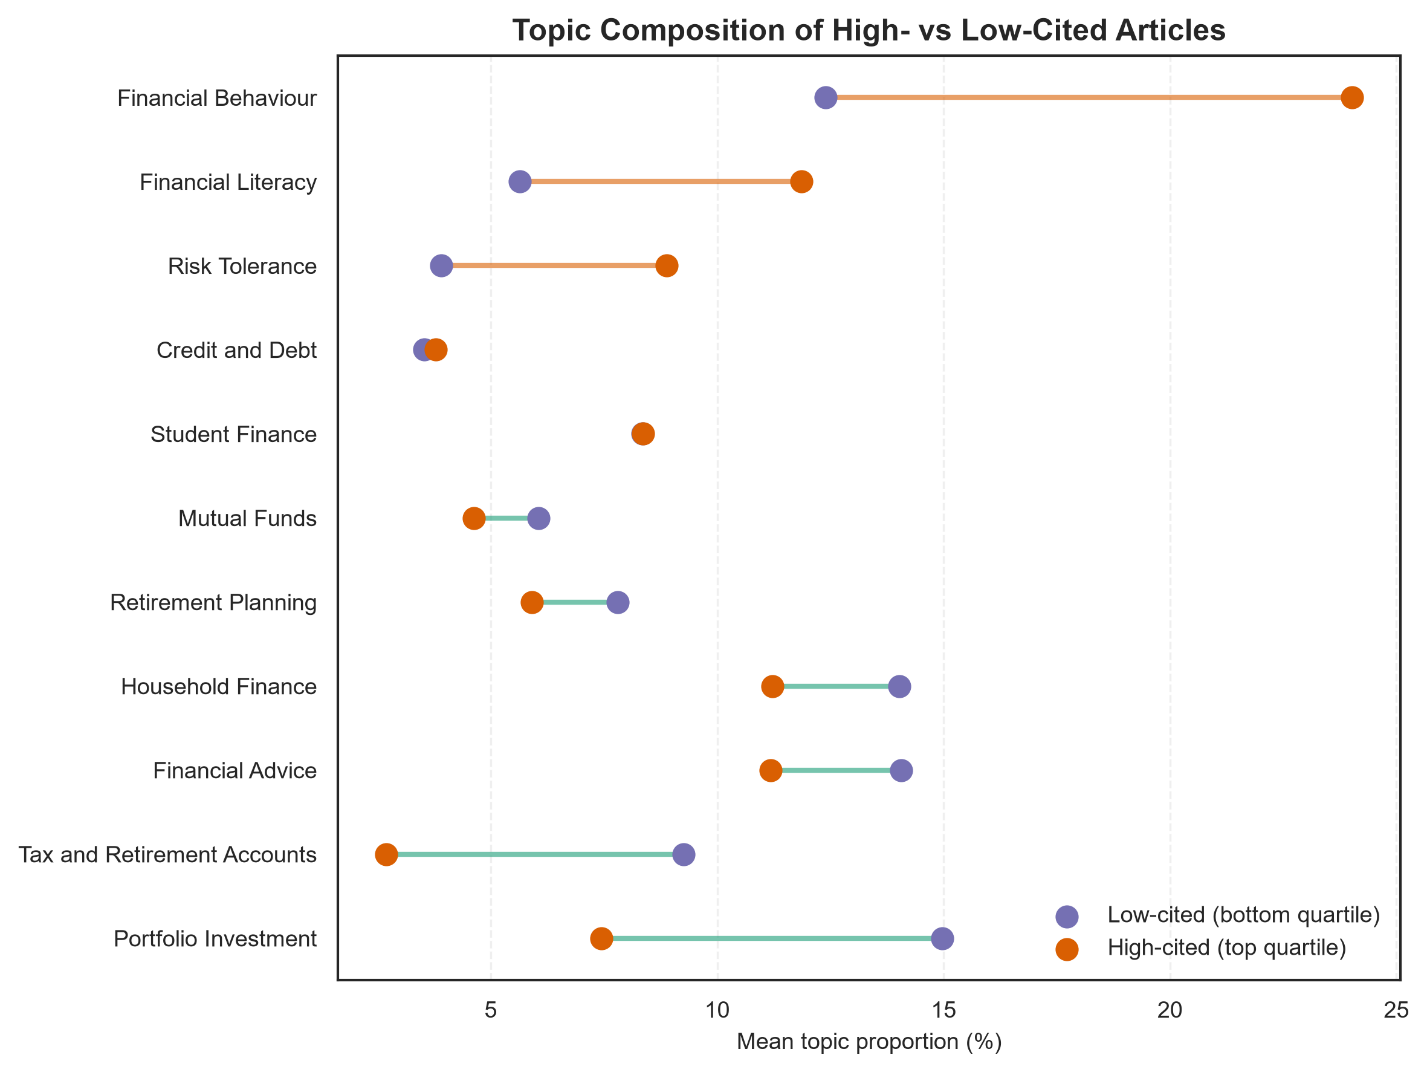
\includegraphics[width=0.75\textwidth]{figures/qb_topic_hilo.png}
\end{figure}

\subsubsection{FSR's topic mix relative to its competitors}\label{qb-opportunity}

To identify topics where FSR could plausibly improve its citation impact, each journal's topic composition was cross-referenced with that topic's citation impact from the regression. For each topic we compared FSR's mean share of articles against the average share of FPR and JFCP, and set that against the topic's IRR. A topic was flagged as an opportunity only if it met both conditions: a statistically significant IRR above 1, indicating the topic is genuinely associated with higher citation rates, and an FSR share below the competitor average, indicating FSR under-publishes in it. Both were required because a topic where FSR trails its competitors is only a meaningful opportunity if that topic is actually associated with higher citations; recommending that FSR imitate a competitor's topic mix without regard to citation impact would not be evidence-based.

\begin{table}[htbp]
\centering
\small
\caption{FSR topic share against competitors, cross-referenced with citation impact}
\label{tab:qb_gap}
\begin{tabular}{lrrrrrl}
\toprule
Topic & FSR (\%) & FPR (\%) & JFCP (\%) & IRR & FSR gap (pp) & Opportunity \\
\midrule
Financial Behaviour & 5.92 & 11.55 & 27.61 & 6.20 & $-13.66$ & Yes \\
Financial Literacy & 6.13 & 7.78 & 8.53 & 9.42 & $-2.03$ & Yes \\
Student Finance & 5.22 & 1.72 & 10.91 & 2.90 & $-1.10$ & Yes \\
Risk Tolerance & 6.17 & 5.49 & 6.55 & 6.65 & 0.15 & No \\
Credit and Debt & 3.84 & 1.90 & 4.86 & 1.81 & 0.46 & No \\
Household Finance & 9.24 & 7.97 & 19.08 & 1.30 & $-4.29$ & No \\
Retirement Planning & 7.89 & 5.46 & 6.58 & 1.00 & 1.87 & No \\
Mutual Funds & 12.01 & 1.62 & 1.94 & 0.86 & 10.23 & No \\
Financial Advice & 10.20 & 45.16 & 6.99 & 0.83 & $-15.87$ & No \\
\bottomrule
\end{tabular}
\tablenote{FSR gap (pp) is FSR's topic share minus the average of FPR and JFCP's shares.}
\end{table}

Three topics met both criteria: Financial Literacy, Financial Behaviour and Student Finance. The gap was largest for Financial Behaviour, where FSR's share (5.92\%) trails JFCP's (27.61\%) by nearly 14 percentage points despite Financial Behaviour carrying the third-highest IRR (6.20) of any topic. Financial Literacy, the topic most strongly associated with citations (IRR = 9.42), shows a smaller but consistent gap (6.13\% against a competitor average of 8.15\%). Student Finance shows a more modest gap, driven mainly by JFCP's larger share (10.91\% against 5.22\%).

Two patterns outside the opportunity criteria are still worth noting. FPR concentrates heavily on Financial Advice (45.16\% against FSR's 10.20\%), but with an IRR of 0.83 that concentration is not associated with higher citations. FSR shows the opposite pattern in Portfolio Investment, where it leads all three journals (23.27\%) despite that topic's low IRR (0.51), which suggests effort directed at a theme with limited citation payoff.

\begin{figure}[htbp]
\centering
\caption{Topic share by journal. Shaded rows indicate topics meeting both opportunity criteria.}
\label{fig:qb_journal}
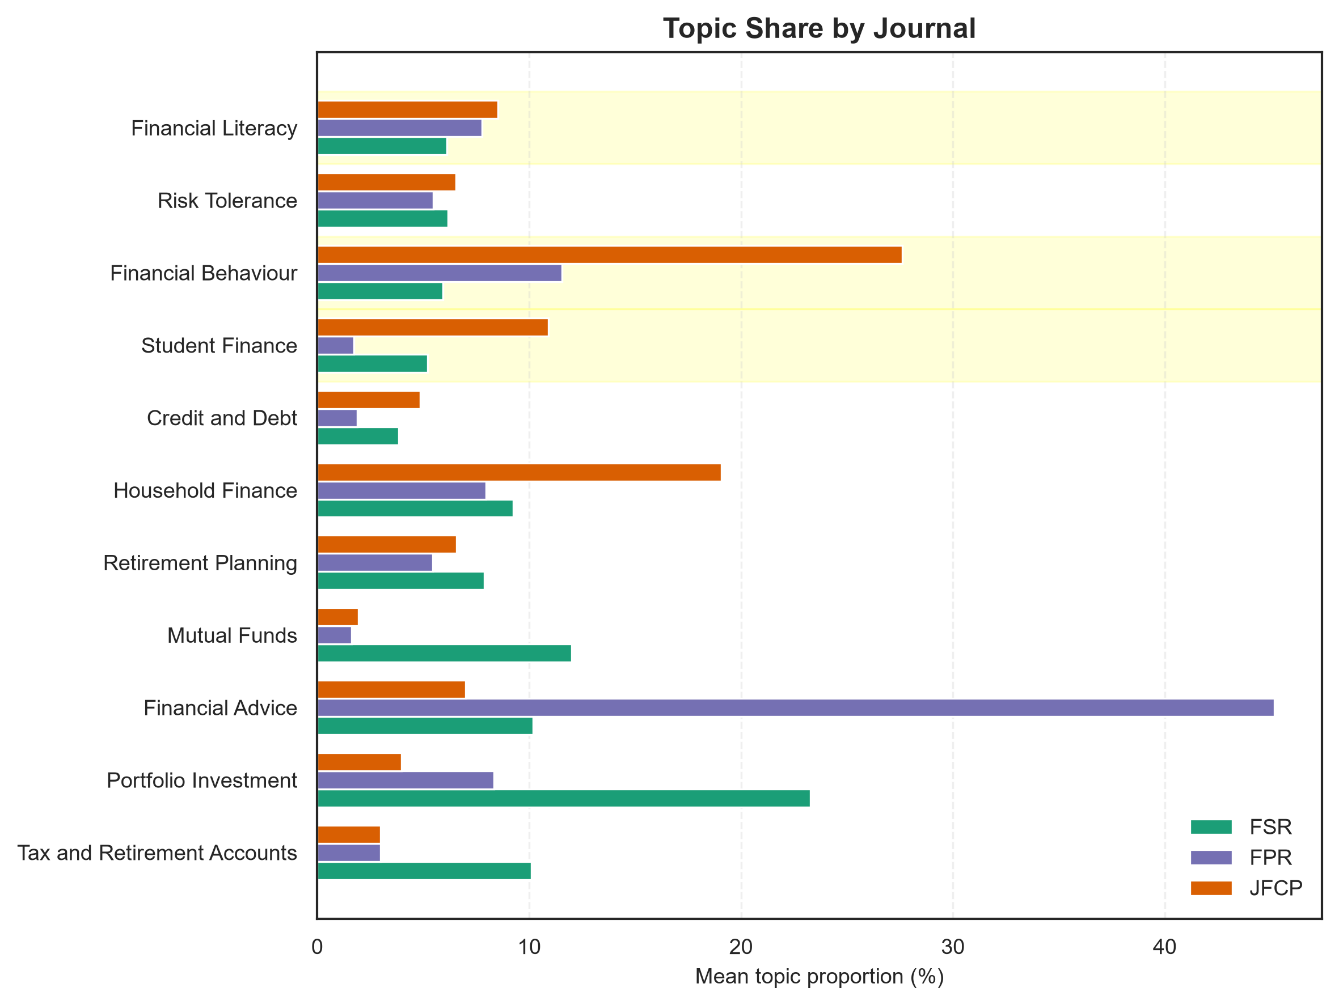
\includegraphics[width=0.75\textwidth]{figures/qb_topic_by_journal.png}
\end{figure}

Over the past five years (2021--2025), Financial Behaviour showed the largest increase in prevalence, rising from 26.6\% to 28.4\% of articles (+1.29 percentage points per year), while Financial Literacy showed the largest decrease, falling from 13.4\% to 9.6\% ($-1.32$ percentage points per year). Neither trend was statistically significant after correcting for multiple comparisons across the eleven topics (Financial Behaviour: \(p_{adj}\) = .62; Financial Literacy: \(p_{adj}\) = .58), so these should be read as the two largest observed movements over the period rather than confirmed trends. With only five annual observations per topic this analysis has limited power; a longer window was not used because FPR did not begin publishing until 2018, which would introduce composition effects into an extended pooled trend.

\begin{figure}[htbp]
\centering
\caption{Recent topic trends, 2021--2025.}
\label{fig:qb_trends}
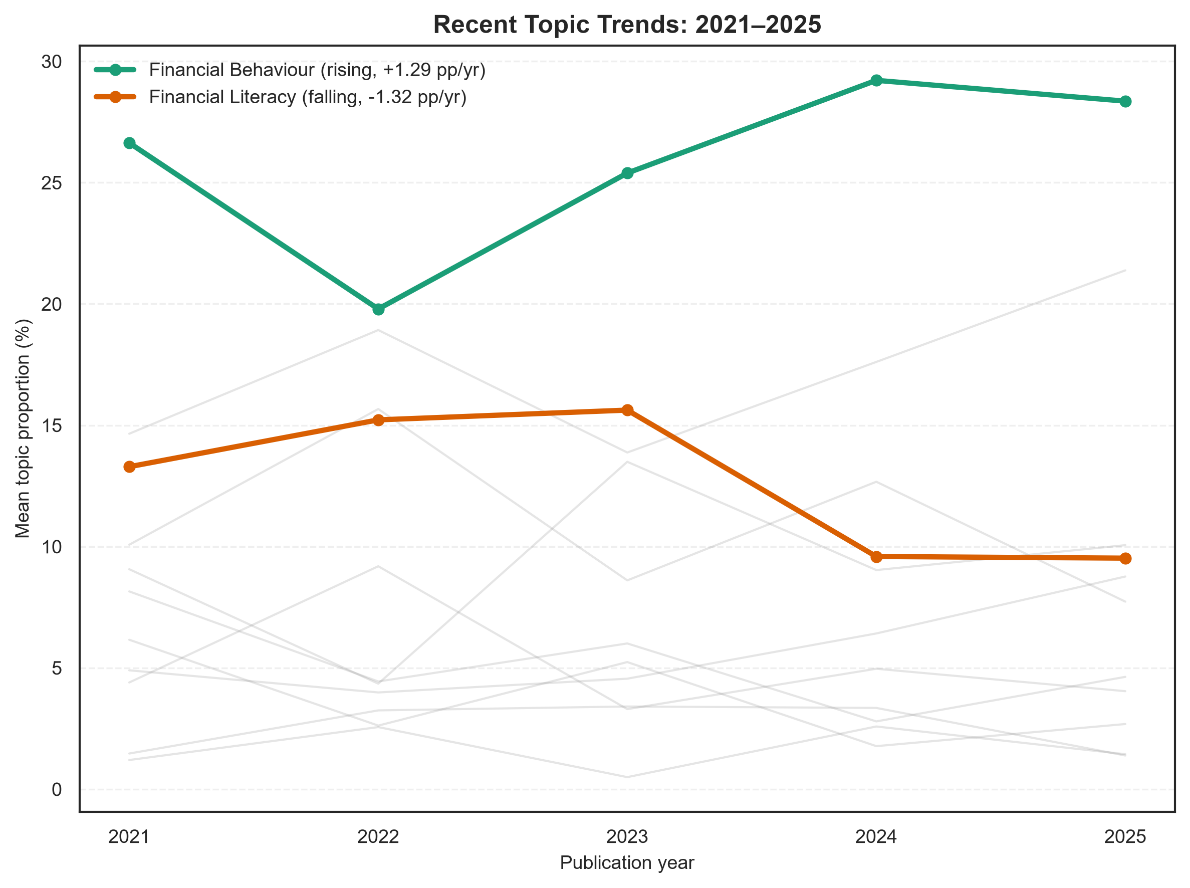
\includegraphics[width=0.75\textwidth]{figures/qb_trends.png}
\end{figure}

\subsection{Question C: Does a Clearly Written Abstract Get Cited More?}\label{question-c-does-a-clearly-written-abstract-get-cited-more}

Abstracts in all three journals are demanding to read. Mean Gunning Fog scores sit between 19.8 and 21.1, which corresponds to roughly postgraduate reading level, and the three journals differ (Kruskal--Wallis \(H\) = 21.82, \(p < .001\)). FSR publishes the most readable abstracts of the three on every measure, though the margin is small relative to the spread within each journal.

\begin{table}[htbp]
\centering
\small
\caption{Abstract readability by journal}
\label{tab:qc_desc}
\begin{tabular}{lrrrrr}
\toprule
Journal & $n$ & Fog mean (SD) & Flesch Reading Ease & Flesch-Kincaid & Words \\
\midrule
FSR & 622 & 19.8 (3.4) & 20.7 & 16.0 & 116 \\
JFCP & 622 & 20.5 (3.4) & 16.6 & 16.7 & 117 \\
FPR & 109 & 21.1 (3.1) & 12.5 & 17.4 & 157 \\
\bottomrule
\end{tabular}
\tablenote{Higher Fog and Flesch-Kincaid scores indicate harder text; higher Flesch Reading Ease indicates easier text. Kruskal--Wallis test across the three journals: $H = 21.82$, $p < .001$.}
\end{table}

Unadjusted, readability has no apparent relationship with citations in any journal: the Spearman correlation between Fog score and citation count is \(-0.05\) in FSR (\(p\) = .27) and \(+0.01\) in JFCP (\(p\) = .78). In FPR it is \(-0.22\) (\(p\) = .03), pointing the opposite way to the adjusted estimate below. These nulls are misleading, because Fog scores are negatively correlated with article age in every journal (\(\rho\) = \(-0.26\) in FSR, \(-0.33\) in JFCP and \(-0.21\) in FPR). Older articles are simultaneously more readable and more cited, so age suppresses the association until it is controlled.

Once age, team size and journal are controlled, the pooled model reproduces the expected result: each additional Fog point is associated with 6.8\% more citations (IRR = 1.068, 95\% CI 1.045--1.091, \(p < .001\)). Taken alone, that is the headline result. Among the controls, article age dominates (IRR = 3.529, 95\% CI 3.192--3.902) and team size carries a small positive association (IRR = 1.092, 95\% CI 1.026--1.163, \(p\) = .006), which is the figure Question D compares against. Variance inflation factors are low for Fog, age and team size (all below 1.4); the two journal indicators carry VIFs of 4.3 (FSR) and 4.1 (JFCP), below the conventional threshold of 5 but close enough to note, for the same reason Question B's journal indicators sit just above it: journal and the variables that differ by journal are not fully independent. The dispersion parameter is \(\alpha\) = 1.502 (SE = 0.057, \(p < .001\)), confirming the overdispersion that motivates the negative binomial specification.

\begin{table}[htbp]
\centering
\small
\caption{Pooled negative binomial models of citation count on abstract readability}
\label{tab:qc_models}
\begin{tabular}{llrrr}
\toprule
Model & Readability measure & IRR & 95\% CI & p-value \\
\midrule
Main adjusted model & Gunning Fog Index & 1.068 & 1.045--1.091 & $<$ .001 \\
+ Abstract length & Gunning Fog Index & 1.068 & 1.045--1.091 & $<$ .001 \\
+ Abstract length & Flesch Reading Ease & 0.983 & 0.978--0.988 & $<$ .001 \\
+ Abstract length & Flesch-Kincaid Grade & 1.060 & 1.033--1.089 & $<$ .001 \\
+ Abstract length and research topic & Gunning Fog Index & 1.045 & 1.024--1.067 & $<$ .001 \\
\bottomrule
\end{tabular}
\tablenote{IRR = incidence rate ratio; CI = confidence interval. All models control for $\log(2026-\text{year}+1)$, number of authors and journal. Flesch Reading Ease runs in the opposite direction to the other two measures, so an IRR below 1 carries the same meaning as an IRR above 1 for Fog.}
\end{table}

That pooled estimate conceals most of what matters. Fitting the same model separately within each journal shows that the association is carried almost entirely by JFCP, where a Fog point is worth 9.5\% more citations, and by FPR at 8.3\%. In FSR the estimate is 3.4\%, half the pooled figure, and its confidence interval includes no effect (\(p\) = .059).

\begin{table}[htbp]
\centering
\small
\caption{The Gunning Fog association, estimated separately within each journal}
\label{tab:qc_strat}
\begin{tabular}{lrrrr}
\toprule
Journal & $n$ & IRR & 95\% CI & p-value \\
\midrule
FSR & 622 & 1.034 & 0.999--1.071 & .059 \\
JFCP & 622 & 1.095 & 1.064--1.126 & $<$ .001 \\
FPR & 109 & 1.083 & 1.001--1.173 & .047 \\
\bottomrule
\end{tabular}
\tablenote{Each model controls for $\log(2026-\text{year}+1)$ and number of authors within the journal concerned. The pooled estimate across all three journals is 1.068 (1.045--1.091).}
\end{table}

The difference between journals is larger than sampling noise. Adding a readability-by-journal interaction to the pooled model improves fit significantly (LR \(\chi^2(2)\) = 8.19, \(p\) = .017), so a single slope does not describe all three journals. Taking FSR as the baseline, JFCP's slope is significantly steeper (ratio = 1.064, 95\% CI 1.020--1.111, \(p\) = .004), while FPR's is not distinguishable from FSR's (ratio = 1.029, 95\% CI 0.943--1.122, \(p\) = .524), which is what 109 articles support.

The FSR estimate also fails the robustness checks that JFCP passes. Within FSR, once abstract length is controlled, the Fog association is not significant (IRR = 1.032, \(p\) = .076) and the Flesch-Kincaid measure gives nothing (IRR = 1.028, \(p\) = .193), even though the Flesch Reading Ease measure remains significant. Within JFCP all three measures agree and all three are significant. Within FPR none of the three reaches significance once length is controlled (Table~\ref{tab:qc_robust}, Appendix~\ref{app:qc_qd_supp}).

Adding research topic removes the FSR association altogether. Controlling for the eleven topics from Question B alongside abstract length, the Fog estimate in FSR falls to 1.015 (95\% CI 0.982--1.049, \(p\) = .371), while JFCP retains a clear association at 1.062 (\(p < .001\)) and FPR becomes non-significant at 1.057 (\(p\) = .187). In the pooled model the topic control shrinks the estimate from 1.068 to 1.045 but leaves it significant, which again reflects JFCP's weight in the pooled sample.

\begin{figure}[htbp]
\centering
\caption{Adjusted association between Gunning Fog Index and predicted citation count for FSR articles.}
\label{fig:qc_fog}
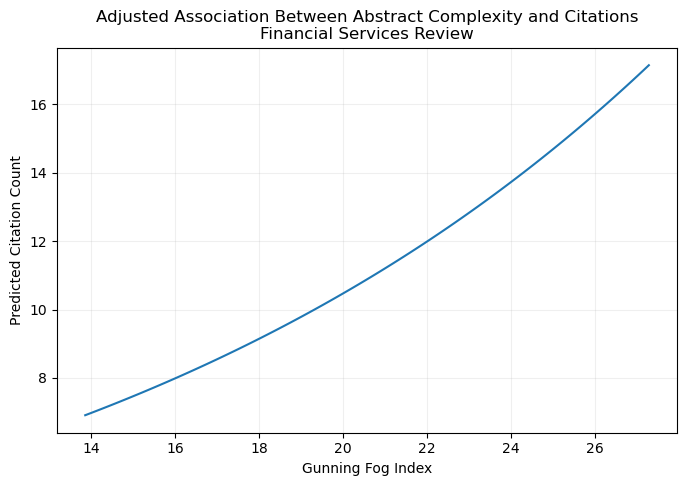
\includegraphics[width=0.65\textwidth]{figures/qc_fog_predicted.png}
\end{figure}

\subsection{Question D: When Does Citation Impact Emerge, and Which Papers Become ``High Hitters''?}\label{question-d-when-does-citation-impact-emerge-and-which-papers-become-high-hitters}

\subsubsection{Part 1: Time to citation peak}\label{part-1-time-to-citation-peak}

Citation impact at FSR builds slowly rather than immediately. The typical (median) paper takes about 7 years to reach its observed citation peak, and there is wide variation around that: the middle half of papers peak between 3 and 11 years after publication, and the mean peak age is 8.1 years. Only 18.8\% of papers have reached their peak by year 2 and 43.7\% by year 5, so a short citation window describes early momentum rather than mature influence.

\begin{table}[htbp]
\centering
\small
\caption{Estimated Time to Citation Peak (Kaplan--Meier Quantiles)}
\label{tab:qd_quantiles}
\begin{tabular}{lr}
\toprule
Quantile & Peak age (years) \\
\midrule
25th percentile & 3 \\
Median (50th) & 7 \\
75th percentile & 11 \\
\bottomrule
\end{tabular}
\tablenote{Estimated from the 442 FSR articles with a retrievable citation history, of which 376 reached an observed peak and 66 remained censored.}
\end{table}

\begin{figure}[htbp]
\centering
\caption{Half of FSR papers reach their observed citation peak within seven years, but the spread around that is wide.}
\label{fig:qd_km}
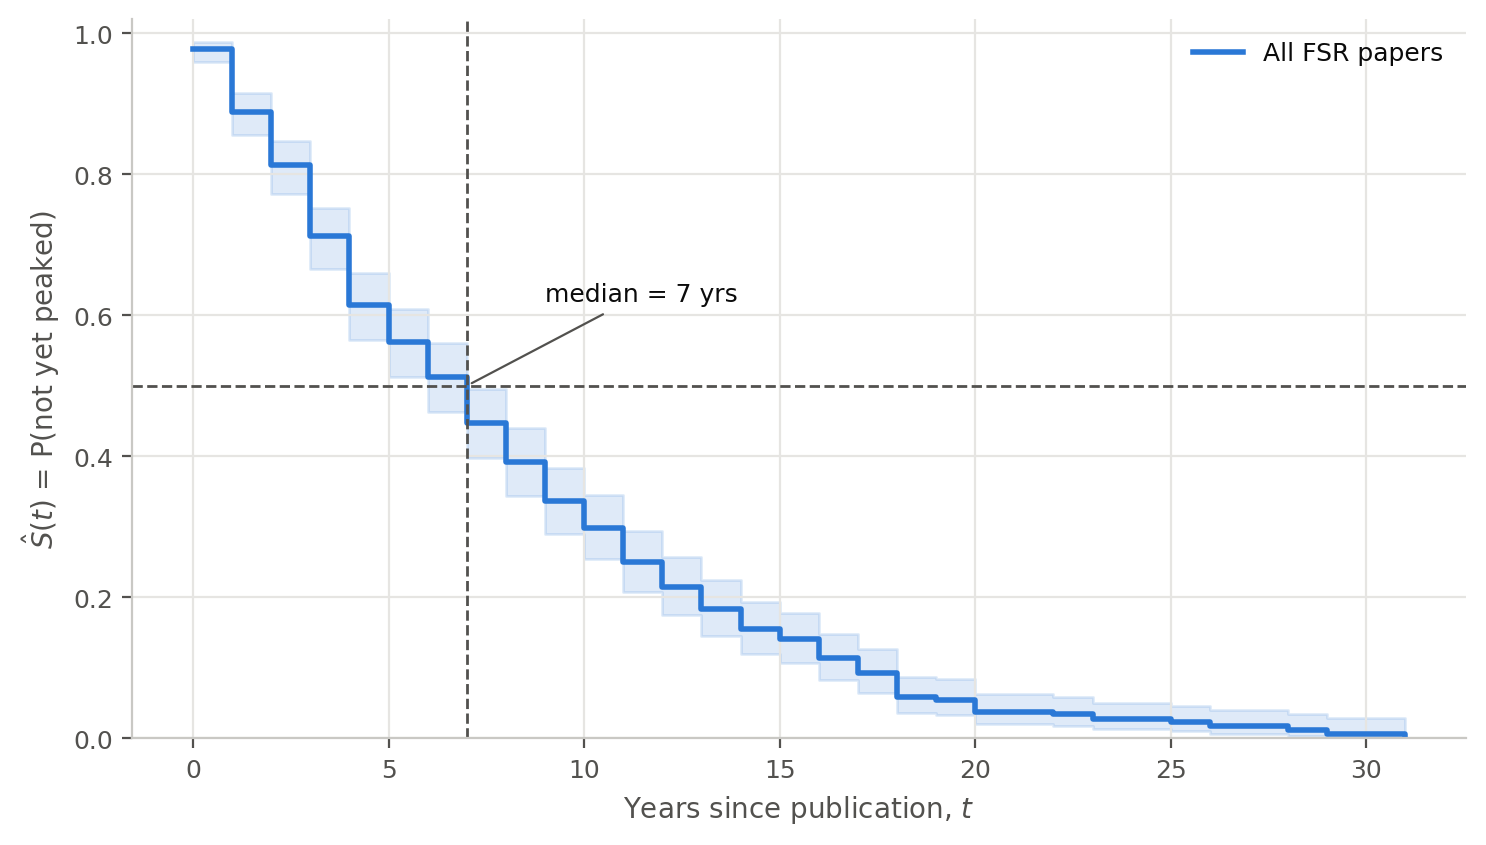
\includegraphics[width=0.65\textwidth]{figures/qd_km_overall.png}
\end{figure}

Peak timing has moved earlier, although by less than a first comparison suggests. Measured over the full available history, median peak age falls from 10 years for the 1990s cohort to 7 years for the 2000s and 4 years for papers published from 2010 onward, and the three distributions differ (log-rank $p < .001$; curves in Appendix~\ref{app:qc_qd_supp}, Figure~\ref{fig:qd_era}). That comparison is not like for like. The recent cohort has been observed for a much shorter period and cannot record a late peak, so part of the gap is a property of the observation window rather than of citation behaviour.

The landmark analysis in Table~\ref{tab:qd_landmark} removes this problem by observing every era over the same eight-year window. The difference that survives is between the 1990s and the 2000s, where median peak age falls from 6 years to 5 ($p = .014$). The 2000s and the 2010s onward are indistinguishable ($p = .97$). The evidence therefore supports a single shift in peak timing between the 1990s and the 2000s, which is consistent with the move to online indexing and full-text search, rather than a continuing acceleration.

\begin{table}[htbp]
\centering
\small
\caption{Time to Citation Peak by Era Over a Common Observation Window}
\label{tab:qd_landmark}
\begin{tabular}{lrrr}
\toprule
Era & $n$ & Peaked by year 8 & Median peak age \\
\midrule
1990s (1991--1999) & 109 & 66.1\% & 6 \\
2000s (2000--2009) & 143 & 81.1\% & 5 \\
2010s+ (2010--2017) & 104 & 78.8\% & 4 \\
\bottomrule
\end{tabular}
\tablenote{Every era is observed over the same eight-year window, so an observed peak means the same thing in each group; an article is included only if it is at least eight years old. An eight-year window leaves at least 104 articles in every era, which is enough for the comparison to be informative. Overall log-rank: $\chi^2(2) = 6.97$, $p = .031$. Pairwise: 1990s against 2000s $p = .014$, 2000s against 2010s+ $p = .97$.}
\end{table}

\subsubsection{Part 2: What makes a paper a high hitter}\label{part-2-what-makes-a-paper-a-high-hitter}

Citations at FSR are highly concentrated in a small number of papers: the top 10\% of papers account for close to two-thirds of all citations in the journal, while the bottom half contribute only a small fraction. This means that being able to recognise a likely high hitter, even imperfectly, would be valuable for editorial strategy.

After controlling for paper age, the number of authors is the clearest bibliographic signal: each additional author on a paper was associated with 1.56 times the odds of it becoming a high hitter (95\% CI 1.10--2.19, $p = .011$). That estimate is sensitive to which controls are present, as Table~\ref{tab:qd_specs} (Appendix~\ref{app:qc_qd_supp}) sets out. Paper age itself was, as expected, also strongly associated with high-hitter status, since older papers have simply had more time to accumulate citations. None of the other characteristics examined (number of affiliations, number of keywords, page length or abstract length) showed a statistically reliable association.

\begin{table}[htbp]
\centering
\small
\caption{Logistic Regression of High-Hitter Status}
\label{tab:qd_logit}
\begin{tabular}{lrrr}
\toprule
Feature & Odds ratio & 95\% CI & p-value \\
\midrule
log(age) & 4.33 & 1.96--9.56 & $<$ .001 \\
Number of authors & 1.56 & 1.10--2.19 & .011 \\
Number of affiliations & 0.70 & 0.47--1.05 & .086 \\
Abstract length & 0.99 & 0.98--1.00 & .095 \\
Page length & 1.05 & 0.99--1.11 & .135 \\
Number of keywords & 1.03 & 0.87--1.21 & .769 \\
\bottomrule
\end{tabular}
\tablenote{OR = odds ratio; CI = confidence interval. The model controlled for log-transformed paper age, number of authors, number of affiliations, number of keywords, page length and abstract length. $n = 582$, of which 63 are high hitters.}
\end{table}

\begin{figure}[htbp]
\centering
\caption{Team size is the clearest paper characteristic linked to becoming a high hitter, once paper age is accounted for.}
\label{fig:qd_or}
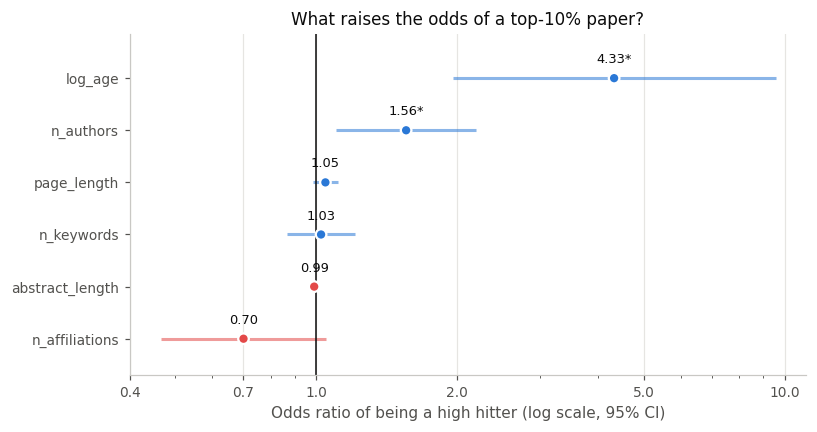
\includegraphics[width=0.65\textwidth]{figures/qd_odds_ratios.png}
\end{figure}

In practical terms, two additional authors multiply the odds of high-hitter status by 2.42, which for a paper at the sample mean on every other characteristic raises the predicted probability from 4.5\% with one author to 10.3\% with three. When the model was tested on how well it picks out individual high-hitter papers, however, its performance was only modestly better than chance. Cross-validated AUC was 0.687, against 0.666 for paper age on its own, and at a threshold flagging the top 10\% of predicted papers the model recovered 13 of the 63 actual high hitters. Adding research topic raises cross-validated AUC to 0.787 and recovers 29 of 63, which places the limitation in the bibliographic variables rather than in the method. Even with topic included more than half of the high hitters are missed, so these variables cannot reliably predict which paper will become a breakout success.

The model does better than random guessing at spotting high-hitter papers, but not by a wide margin (ROC curve in Appendix~\ref{app:qc_qd_supp}, Figure~\ref{fig:qd_roc}): bibliographic metadata alone has limited predictive power.

Table~\ref{tab:qd_specs} (Appendix~\ref{app:qc_qd_supp}) reports how the author association behaves under different specifications and on both outcome scales, and two points follow. First, the estimate in Table~\ref{tab:qd_logit} depends on the presence of the affiliation count. With that variable removed the association weakens to $p = .071$, and neither variable is significant on its own. The two are correlated at $r = 0.61$, because the affiliation field records one entry per author, so they compete to explain the same variation in team size. Once research topic is controlled the association strengthens on both scales in the full specification, to an odds ratio of 1.77 ($p = .003$) and an incidence rate ratio of 1.33 ($p < .001$), although in the sparsest logistic specification, with age and authors alone alongside topic, it falls to $p = .070$. The count-scale estimate remains significant in every specification tested.

Second, the odds ratio of 1.56 corresponds to an incidence rate ratio of 1.24 on the citation count, using the same sample and the same controls, and 1.33 once topic is added. An odds ratio defined on a top-decile outcome always sits further from 1 than the rate ratio describing the same underlying relationship, so the two are not alternative estimates of one quantity. The count-scale figure is the one that can be compared with the incidence rate ratios reported under Questions A and C.

Because the high-hitter result rests on a single threshold, the same six characteristics were re-examined using quantile regression, which describes the relationship at different points of the citation distribution without needing a cutoff at all. Paper age was significant at every point of the distribution, as expected, and author count was significant from the 25th percentile upward, both consistent with the logistic regression result. None of the remaining four characteristics (affiliations, keywords, page length, abstract length) reached significance at any point of the distribution.

The coefficient on author count rises from 0.173 at the median to 0.276 at $\tau$ = 0.90, which would suggest the association is concentrated among the most-cited papers. That difference does not survive testing. Across 600 bootstrap replicates it is $+0.103$, with a 95\% confidence interval of $-0.209$ to $+0.316$ ($p = .62$). Refitting the logistic model at successively more extreme thresholds gives the same answer: odds ratios of 1.40 for the top half, 1.38 for the top quartile, 1.56 for the top decile and 1.31 for the top 5\%, the last of which is not significant. Team size is therefore associated with citations at a broadly constant rate across the distribution rather than mainly at the top, a pattern that holds across quantiles for every feature tested (full per-quantile $p$-values in Table~\ref{tab:qd_qr}, Appendix~\ref{app:qc_qd_supp}).

\section{Discussion}\label{discussion}

\subsection{Question A: Do Star Authors Drive Citations?}\label{question-a-do-star-authors-drive-citations-1}

FSR\textquotesingle s citations are concentrated, but the concentration is not evidence of a small elite of authors carrying the journal. The comparator journals show the same figures, so this is the shape of the field rather than something FSR does differently. More telling, inequality across FSR authors is identical to inequality across FSR articles, and three quarters of FSR authors have published in the journal once. The statistic that the top 10\% of authors hold 66\% of citations is true and will remain true, but it is the arithmetic consequence of a heavy-tailed citation distribution seen through the author list, and it says less about author quality than it appears to. JFCP is the one journal where an author effect is visible, as a gap between its article-level and author-level Gini coefficients, and it arises from a core of authors who return to the journal many times. FSR has no such group. Whether cultivating one would raise citations, or whether JFCP\textquotesingle s returning authors are a consequence of its higher visibility rather than a cause, cannot be settled from citation counts alone.

Prolific, well-known and highly cited are three different groups of people. An editor asked to name FSR's star authors would name different people depending on which definition was used, and the top-20 lists overlap by only three to six names. Where author standing is weighed at all, the modelling suggests prior citations carry the signal, and that the signal is modest: about 18\% more expected citations for a co-author whose h-index is 10 points higher, or about 8\% for a doubling of prior citations, against a multiplier of about 2.6 for a doubling of article age and of about 7 for a financial literacy topic. The holdout test gives the same picture. Knowing the authors' full careers improves the ranking of unseen articles from a correlation of 0.26 to 0.30, which is better than random but a long way from reliable, and every version of the model accounts for little of the variation in citation counts. Recruiting well-known names for special issues or invited papers is therefore a weak lever on citations; a well-cited author is a mild positive signal rather than a safe bet.

The lever that is visible in this data is topical, and it links directly to Question B, whose topic model this analysis shares. FSR's most-cited topics, risk tolerance and financial literacy, are among those it publishes least. Portfolios and markets, mutual funds, tax and withdrawals and retirement saving together make up more than half of FSR's articles, are its least cited, and cannot be told apart from one another in the citation model. This is not a case for abandoning the investment and retirement literature, which is core to the field, but it is where the largest measurable differences in citation performance sit. The pooled model adds a second consideration: with age, topic and authorship held constant, the same article is expected to attract 1.7 times the citations in JFCP and 2.0 times in FPR, so the journal's own visibility matters at least as much as who wrote the paper.

Several limitations qualify these results. The h-index is a 2026 snapshot and includes reputation earned after an article appeared, which is why the point-in-time prior-citation measure, with its smaller effect, is the better estimate of the forward-looking signal. Citations were whole-counted and self-citations could not be separated out, since Scopus supplies only a total per article; both choices bias towards finding an author effect, and only a weak one was found. Topics come from an unsupervised model and each article is assigned to its single largest topic, so some assignments follow vocabulary rather than subject, as with the two financial literacy studies placed under students and loans. Author matching is imperfect: 8.5\% of authors have no OpenAlex record, 53 matched profiles appear to merge several people, and a small number are matched to fragmentary profiles that understate the author's standing, as with Robert W. Faff in Table~\ref{tab:qa_top}. OpenAlex resolves only 81\% of the JFCP articles in the corpus, so the pooled comparison is the least reliable estimate reported here; the FSR-only results do not depend on it. Career statistics come from OpenAlex and article citation counts from Scopus, and the two indexes do not count identically, which affects the size of the track-record effects rather than their direction.

\subsection{Question B: Which Topics Attract Citations, and Where Is FSR Thin?}\label{question-b-which-topics-attract-citations-1}

The topic analysis provides the clearest actionable lever identified in this project. Where Question A found that authorship characteristics explain very little of FSR's citation variation, the topic-proportion model explains substantially more, and the pattern is consistent across three independent analyses: the regression coefficients, the raw topic composition of high- versus low-cited articles, and the cross-journal comparison of topic share. Financial Literacy, Risk Tolerance and Financial Behaviour each carry large, statistically significant incidence rate ratios (9.4, 6.7 and 6.2 respectively) and are over-represented among FSR's most-cited articles relative to its least-cited ones. Of those three, Financial Literacy and Financial Behaviour are also the themes where FSR under-publishes relative to FPR and JFCP; Risk Tolerance is not, since FSR's share of it already matches the competitor average, so the third under-published topic is Student Finance. Three separate ways of looking at the data converge on the same three opportunity topics, Financial Literacy, Financial Behaviour and Student Finance, which is what makes this a defensible recommendation rather than an artefact of one model specification.

The choice of NMF with eleven topics over LDA and BERTopic should be read as a pragmatic decision rather than a claim that NMF is the correct model. LDA's coherence and perplexity did not converge on a shared optimum, and BERTopic, while capable of surfacing themes the bag-of-words models missed, left over a third of articles unassigned at its best setting and is designed for corpora considerably larger than 1,362 documents. NMF was preferred because it gave complete, interpretable assignment at competitive coherence. The topic labels used across Questions A, B, C and D are therefore one reasonable partition of the corpus rather than a ground truth; a different \(k\) or algorithm could shift articles between adjacent themes such as Financial Behaviour and Household Finance, which is the likely explanation for Household Finance behaving inconsistently between the regression (positive, non-significant) and the raw quartile comparison (lower share among high-cited articles).

Two design choices limit how far the topic-citation relationship can be trusted causally. First, topic proportions are correlational predictors in an observational dataset: a topic being associated with more citations does not mean that publishing more on it would cause FSR's citation rate to rise, since those topics may simply attract more active research communities, larger reference lists, or more citable review-style work for reasons unrelated to editorial choice. Second, the journal indicators carried VIFs of 5.2 to 5.9, just above the conventional threshold, because journals and topics are not independent; JFCP publishes far more Financial Behaviour content than FSR does. This does not invalidate the topic coefficients, but the journal effects reported alongside them should be treated as approximate rather than cleanly separable from topic composition.

The opportunity rule, combining a significant IRR above 1 with a below-competitor topic share, is a simple and transparent decision rule, which is its main strength for an industry audience: AFS's editorial team can see exactly why Financial Behaviour, Financial Literacy and Student Finance were flagged and why Portfolio Investment was not, despite FSR publishing disproportionately in it. The trade-off is that the rule treats each theme independently and ignores interactions, and the gap statistic compares raw article shares rather than citation-weighted ones, so it identifies where FSR is thin in coverage but not how much citation upside closing that gap would deliver. The recent-trend analysis carries the least weight of anything reported here: with five annual observations per topic and no trend surviving correction for multiple comparisons, it is descriptive rather than evidence of a shift in the field.

\subsection{Question C: Does a Clearly Written Abstract Get Cited More?}\label{question-c-does-a-clearly-written-abstract-get-cited-more-1}

The hypothesis that easier abstracts attract more citations is not supported. If anything the pooled association runs the other way: once article age, team size and journal are controlled, more complex abstracts are associated with higher citation counts, and that direction is consistent across all three readability measures. Age is what hides this in the raw data, since older articles are both more readable and more cited, which is why the unadjusted correlations sit near zero in every journal.

The more useful finding is that this association is not FSR's. Estimated within journals, a Gunning Fog point is worth 9.5\% more citations in JFCP and 8.3\% in FPR, but only 3.4\% in FSR, where the interval includes no effect (\(p\) = .059). The interaction test confirms that one slope does not fit all three journals (\(p\) = .017), and that JFCP's slope is significantly steeper than FSR's (\(p\) = .004).

The FSR estimate is also the least robust of the three. It is already non-significant on its own, it is not reproduced by the Flesch-Kincaid measure once abstract length is controlled, and it disappears entirely once research topic is held constant (IRR = 1.015, \(p\) = .371). JFCP's association survives all three checks. The most economical reading is that what looks like a readability effect in FSR is largely a topic effect: technical subfields are both harder to write about plainly and differently cited, and once those subfields are accounted for the readability signal in FSR is gone. This framing treats topic as a confound to remove, but it could equally be read as a mediator: if subject matter is part of the mechanism by which readability would affect citations, rather than a separate cause of both, controlling for it removes part of the effect under test rather than isolating it from a nuisance variable. The data cannot distinguish these two readings, so the finding is better stated as readability adds nothing once subject matter is held fixed, rather than as proof that readability was never doing anything on its own. That interpretation is consistent with Question B, which finds topic to be the strongest driver of citations in this corpus, and with Question D, where adding topic to a bibliographic model lifts predictive performance more than any individual article characteristic.

Why the association is real in JFCP but not in FSR cannot be settled from these data. One possibility is composition: JFCP publishes far more in the behavioural and literacy themes, where the gap between technical and accessible writing may be wider. Another is audience, since a journal read more heavily by practitioners may reward different writing from one read mainly by academics. Distinguishing these would require readership or download data that the bibliographic record does not contain.

Three limitations qualify all of this. The analysis is observational, so none of these associations licenses a causal claim, and in particular nothing here suggests that making an abstract harder to read would increase its citations. Readability formulas are crude proxies for clarity: they count syllables and sentence length, and a well-written technical abstract and a badly written one can score identically, which is the same limitation Gazni (2011) notes. The FPR estimates rest on 109 articles and should be treated as indicative only.

For AFS the practical implication is narrow but clear. Abstract readability is not a lever for FSR. The pooled result that appears to support one is driven by a comparator journal, and the FSR-specific estimate does not survive controlling for what the articles are about. Editorial effort is better spent on the topic mix identified under Question B than on the prose style of abstracts, and the readability scores reported here are better used as a descriptive characteristic of the journal than as a target to manage.

\subsection{Question D: When Does Citation Impact Emerge, and Which Papers Become ``High Hitters''?}\label{question-d-when-does-citation-impact-emerge-and-which-papers-become-high-hitters-1}

Citation impact at FSR is a long-cycle process. Articles typically take about seven years to reach their observed citation peak, and the middle half take between three and eleven years. Evaluating FSR articles, or the journal itself, on a two- to three-year citation window therefore captures early momentum rather than mature influence and undervalues work whose impact builds gradually. Peak timing has moved earlier over the journal's history, but once each cohort is observed over a common window that shift sits between the 1990s and the 2000s, with no further change since. The journal is not on a continuing acceleration that would justify a shorter evaluation window.

A small group of articles accounts for a disproportionate share of FSR's citations, which makes identifying likely high hitters editorially valuable. Basic bibliographic metadata cannot do this reliably. Author-team size is the clearest signal in the bibliographic record, and the quantile regression shows the association holds across the citation distribution rather than only among the most-cited articles. The apparent strengthening towards the top, where the coefficient rises from 0.173 at the median to 0.276 at the 90th percentile, does not survive a bootstrap test ($p = .62$). The model identifies only 13 of 63 true high hitters and adds little beyond article age, so team size describes a pattern rather than providing a formula for selecting future high-impact articles. Adding research topic raises this to 29 of 63 and lifts cross-validated AUC from 0.687 to 0.787, which locates the limitation in the variables rather than in the method. The other characteristics examined (affiliations, keywords, page length and abstract length) show no reliable association and should not be used as editorial criteria.

The team-size result needs to be read alongside Question A, which reports no detectable effect of co-author count on FSR citations (IRR = 1.062, $p = .318$). The two findings are reconcilable. The headline figures are measured on different scales, and expressing the present result on the citation count gives IRR = 1.24, which sits beside Question A's 1.062 and Question C's 1.092 rather than contradicting them. Controlling for the same eleven topics Question A uses, in a model with age and team size alone, brings the two estimates closer still, to 1.15 here against Question A's 1.062. Question A also measures author standing as the maximum over an article's co-authors of prior works, prior citations and h-index. A maximum over $k$ values rises with $k$ by construction, so a larger team produces a higher best-co-author statistic even when no individual author is better established, and part of the team-size effect is absorbed by those terms. Question C, which uses no maximum-based measure, reports a positive association of similar size. Research topic does not account for the difference either: in the full specification adding it strengthens the association, from an incidence rate ratio of 1.24 to 1.33, rather than removing it. The position supported across the three analyses is that research topic is the substantial lever and team size a small but real secondary association.

One limitation bounds how far these timing results travel. The annual citation trajectories were reconstructed from OpenAlex for FSR only, so unlike Questions A, B and C this question has no comparator analysis: there is no JFCP or FPR peak-timing curve to set the seven-year median against, and no comparator high-hitter model. A seven-year median is therefore a statement about FSR in absolute terms rather than a finding that FSR is slow or fast relative to its field. Building the comparison would mean reconstructing trajectories for the other two journals, which is feasible for FPR but limited for JFCP, where almost half the articles carry no DOI and so cannot be matched to OpenAlex. Until that is done, the evaluation-horizon recommendation should be read as calibrating FSR against its own history rather than against its competitors.

Taken together, these results have two practical implications for AFS. First, FSR's citation performance should be assessed over a horizon of roughly five to seven years rather than a short post-publication window, and the earlier peak timing of recent articles is not large enough to shorten that. Second, research topic carries more predictive weight than any bibliographic characteristic, so editorial attention is better directed at subject matter, as set out under Question B, than at the shape of the manuscript. Author collaboration is worth noting as a descriptive signal, but encouraging superficial changes to team size, abstract length or article length is not supported by these results. Better identification of future high-impact work would require richer information than the bibliographic record, such as novelty or an article's early citation trajectory.

\section{Conclusion}\label{conclusion}

This analysis examined four potential drivers of citation performance in FSR, each with a corresponding recommendation for the Academy of Financial Services. The strength of evidence for those recommendations varies substantially, and the priority given to each should reflect that variation.

The strongest lever for citation improvement is topic composition. Financial Literacy, Risk Tolerance and Financial Behaviour are associated with citation rates 6.2 to 9.4 times higher than the reference category, controlling for article age and journal. Three topics combine that citation premium with a shortfall against competitors, and those are the opportunities: Financial Literacy, Financial Behaviour and Student Finance. Risk Tolerance is cited well, but FSR already publishes it at the competitor rate, so it offers no gap to close. Financial Behaviour shows the largest gap, with FSR at 5.92\% of articles against JFCP's 27.61\%, despite carrying the third-highest citation impact of any topic studied. Financial Literacy, which is associated with the strongest citation rates overall (IRR = 9.42), trails competitor journals by 2.0 percentage points. Student Finance shows a more modest gap but meets the same criteria. In contrast, FSR devotes nearly a quarter of its articles (23.27\%) to Portfolio Investment, far more than FPR at 8.35\% or JFCP at 3.97\%, despite that topic being associated with roughly half the citation rate of the reference category (IRR = 0.51). By redirecting effort from low-impact investment and retirement topics towards behavioural and literacy content, AFS could align the journal with both citation performance and the research activity of the field.

A second recommendation concerns the timeline for evaluating article performance. FSR papers typically require about seven years to reach their observed citation peak, with the middle half peaking between three and eleven years after publication. Short citation windows capture early momentum rather than mature influence. Only 18.8\% of papers peak within two years and 43.7\% within five. Although peak timing has moved earlier over the journal's history, appearing to suggest a six-year shortening between the 1990s and the 2010s, this difference largely reflects differences in observation window rather than true acceleration in citation behaviour. Once three publication eras are observed over the same eight-year window, the evidence shows a shift between the 1990s and 2000s (p = .014) but no further acceleration since. AFS should evaluate FSR's citation performance on a horizon of approximately five to seven years, consistent with the time required for impact to mature.

Three other investigations identified weaker or non-existent relationships. Author track record carries a modest effect: articles with a co-author whose h-index is 10 points higher attract about 18\% more citations, and each doubling of prior citations corresponds to about 8\% more citations, controlling for topic and age. These associations are real but small relative to the topic effect, and the models containing them account for little of the variation in citation counts. The second author effect, team size, shows a similar pattern on a different scale. Larger teams are associated with higher odds of reaching high-hitter status, with each additional author multiplying the odds by 1.56. However, bibliographic metadata including team size correctly identifies only 13 of 63 true high hitters in the sample, and adding research topic lifts that figure to 29. The practical implication is that editorial emphasis on author standing or team composition is unlikely to move citation rates. Topic is the stronger variable in both analyses: it carries far larger effects than either author measure, and adding it to the high-hitter model improves identification more than any bibliographic characteristic does.

Abstract readability shows no association with citations in FSR itself. A pooled analysis across all three journals indicates that more complex abstracts are associated with higher citation counts, but this effect is driven by JFCP and FPR and does not appear in FSR. The FSR estimate of 3.4\% more citations per Fog point is not significant (p = .059) and vanishes entirely once research topic is controlled. The unadjusted correlations near zero are misleading because older articles are both more readable and more cited, creating a suppression effect; the adjusted estimate correctly identifies a readability signal in the comparator journals but not in FSR. The most economical reading is that what appears to be a readability effect in FSR is actually a topic effect: technical subfields differ both in clarity and in citation rates, and once those differences are accounted for the readability signal disappears. Effort spent improving abstract prose will therefore have limited citation payoff.

In summary, the project identifies one clear opportunity for increasing FSR's citations: shifting the journal's topic balance towards Financial Behaviour, Financial Literacy and Student Finance, the three topics that meet both opportunity criteria, and away from the investment and retirement topics that dominate current output. The evidence for this recommendation is consistent across three separate analyses and is readily actionable by AFS's editorial team. The timing recommendation is also straightforward: evaluate the journal on five to seven year timescales rather than on shorter windows. Author track record, team size and abstract readability matter far less and offer little value as editorial policy levers. Topic composition is the highest-leverage variable identified in this analysis and should be the focus of editorial strategy.

\section{References}\label{references}

\textit{[To be completed.]}
% Works cited in the text that need full entries: Didegah and Thelwall (2013); Gazni (2011);
% Kousha and Thelwall (2024); Roder et al. (2015); Sienkiewicz and Altmann (2016); Wang and Aryani (2025).

\appendix
\section{Appendix A: NMF topic labels and top terms}\label{app:topics}

\begin{table}[htbp]
\centering
\small
\caption{The eleven NMF topics and their highest-weighted terms}
\label{tab:appendix_topics}
\begin{tabular}{rll}
\toprule
\# & Label & Top terms \\
\midrule
0 & Retirement Planning & retirement, saving, plan, retirement planning, age, social security, pension, income, retiree \\
1 & Mutual Funds & fund, mutual, mutual fund, performance, return, investor, fund performance, expense, ratio \\
2 & Financial Literacy & literacy, financial literacy, knowledge, financial education, education, financial knowledge, program, confidence \\
3 & Risk Tolerance & risk, tolerance, risk tolerance, financial risk, measure, investment, aversion, assessment, risk taking \\
4 & Credit and Debt & credit, card, credit card, debt, consumer, credit card debt, card debt, payment, cash \\
5 & Portfolio Investment & portfolio, stock, investor, market, asset, investment, allocation, return, bond \\
6 & Household Finance & household, consumer, survey consumer finance, income, finance, insurance, survey, life \\
7 & Financial Advice & financial planning, planner, financial planner, planning, advice, advisor, client, professional \\
8 & Student Finance & student, college, college student, loan, student loan, course, education, debt \\
9 & Financial Behaviour & behavior, financial behavior, satisfaction, management, socialization, adult, family \\
10 & Tax and Retirement Accounts & tax, ira, withdrawal, rate, account, mortgage, roth, taxable, tax rate \\
\bottomrule
\end{tabular}
\tablenote{Topics are labelled from their top terms. Topic 0 (Retirement Planning) is the reference category in the regression below.}
\end{table}

\section{Appendix B: Supplementary material for Questions C and D}\label{app:qc_qd_supp}

This appendix holds robustness checks and supporting figures referenced from the Question C and Question D Methods and Results, moved here to keep the main text focused on the headline results.

\begin{table}[htbp]
\centering
\small
\caption{Readability associations by journal and measure, controlling for abstract length}
\label{tab:qc_robust}
\begin{tabular}{lrrrrrr}
\toprule
& \multicolumn{2}{c}{Gunning Fog} & \multicolumn{2}{c}{Flesch Reading Ease} & \multicolumn{2}{c}{Flesch-Kincaid} \\
\cmidrule(lr){2-3}\cmidrule(lr){4-5}\cmidrule(lr){6-7}
Journal & IRR & p & IRR & p & IRR & p \\
\midrule
FSR & 1.032 & .076 & 0.983 & $<$ .001 & 1.028 & .193 \\
JFCP & 1.095 & $<$ .001 & 0.983 & $<$ .001 & 1.087 & $<$ .001 \\
FPR & 1.059 & .156 & 0.994 & .570 & 1.029 & .570 \\
\bottomrule
\end{tabular}
\tablenote{Each cell is a separate negative binomial model controlling for $\log(2026-\text{year}+1)$, number of authors and abstract length within that journal. Flesch Reading Ease is reversed in direction, so values below 1 indicate the same association as values above 1 for the other two measures. Referenced from Question C Results.}
\end{table}

\begin{figure}[htbp]
\centering
\caption{The pooled readability association is carried by JFCP and FPR rather than by FSR, whose interval reaches down to no effect. Numeric values in Table~\ref{tab:qc_strat}.}
\label{fig:qc_journal}
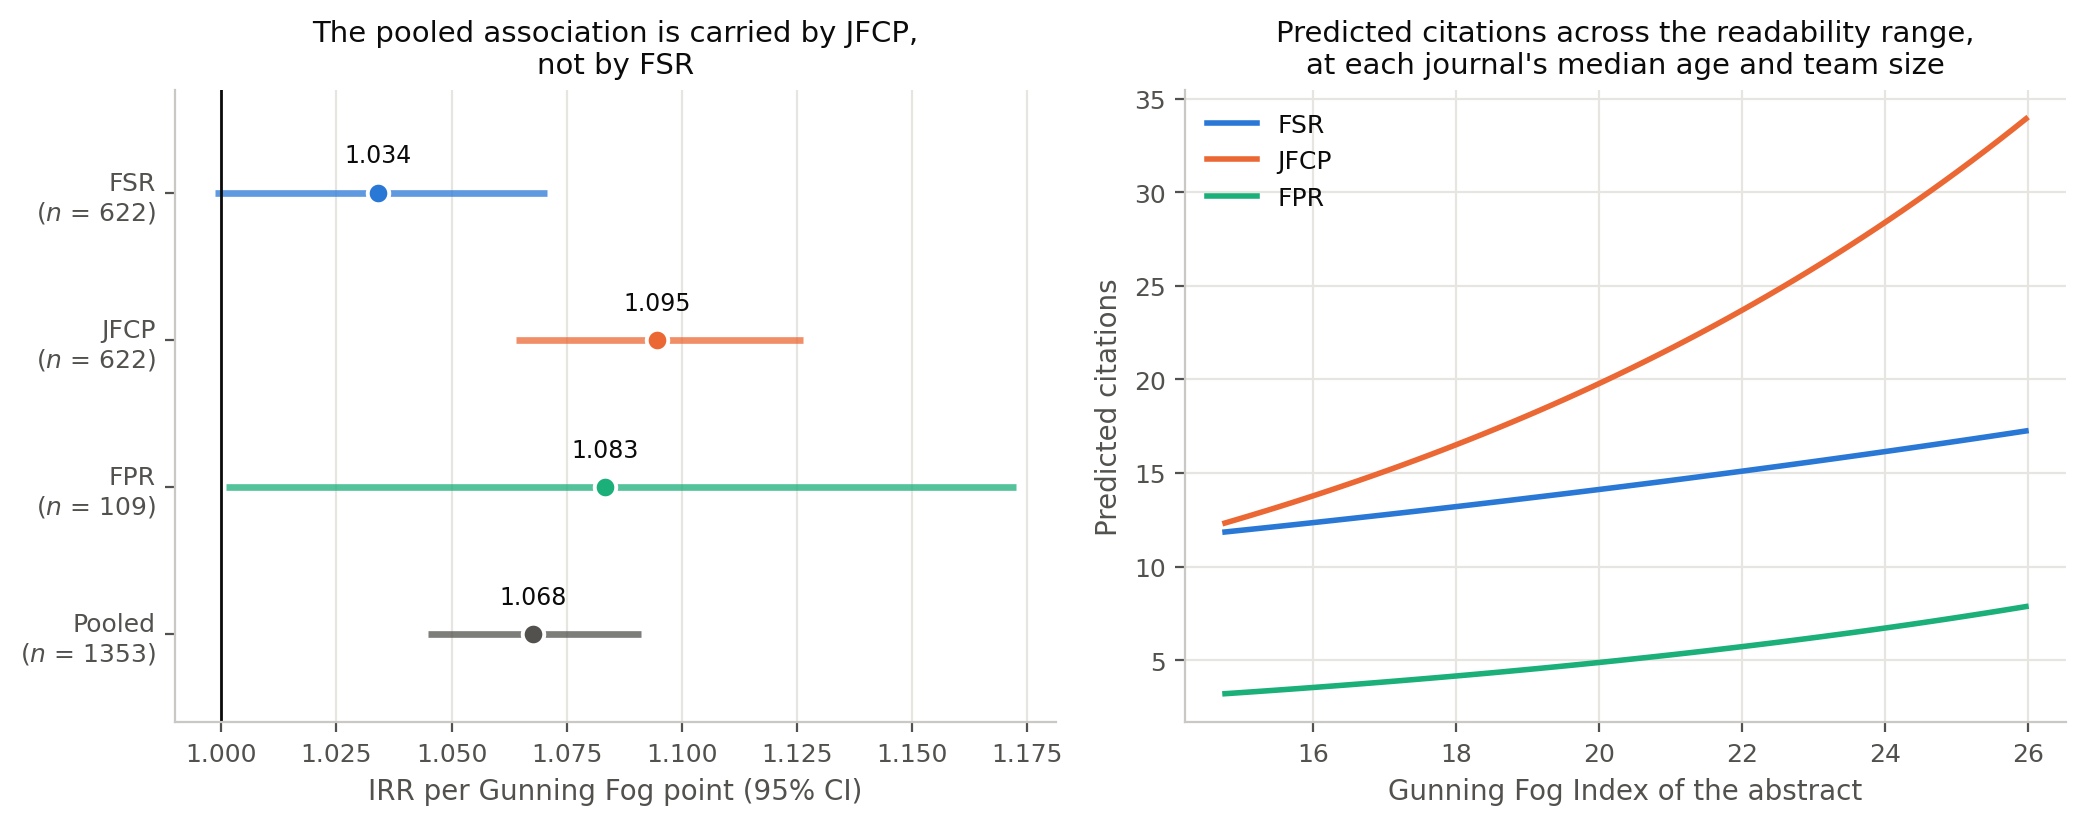
\includegraphics[width=0.8\textwidth]{figures/qc_journal_comparison.png}
\end{figure}

\begin{figure}[htbp]
\centering
\caption{The gap between eras narrows sharply once every cohort is observed over the same eight-year window. Quantified in Table~\ref{tab:qd_landmark}.}
\label{fig:qd_era}
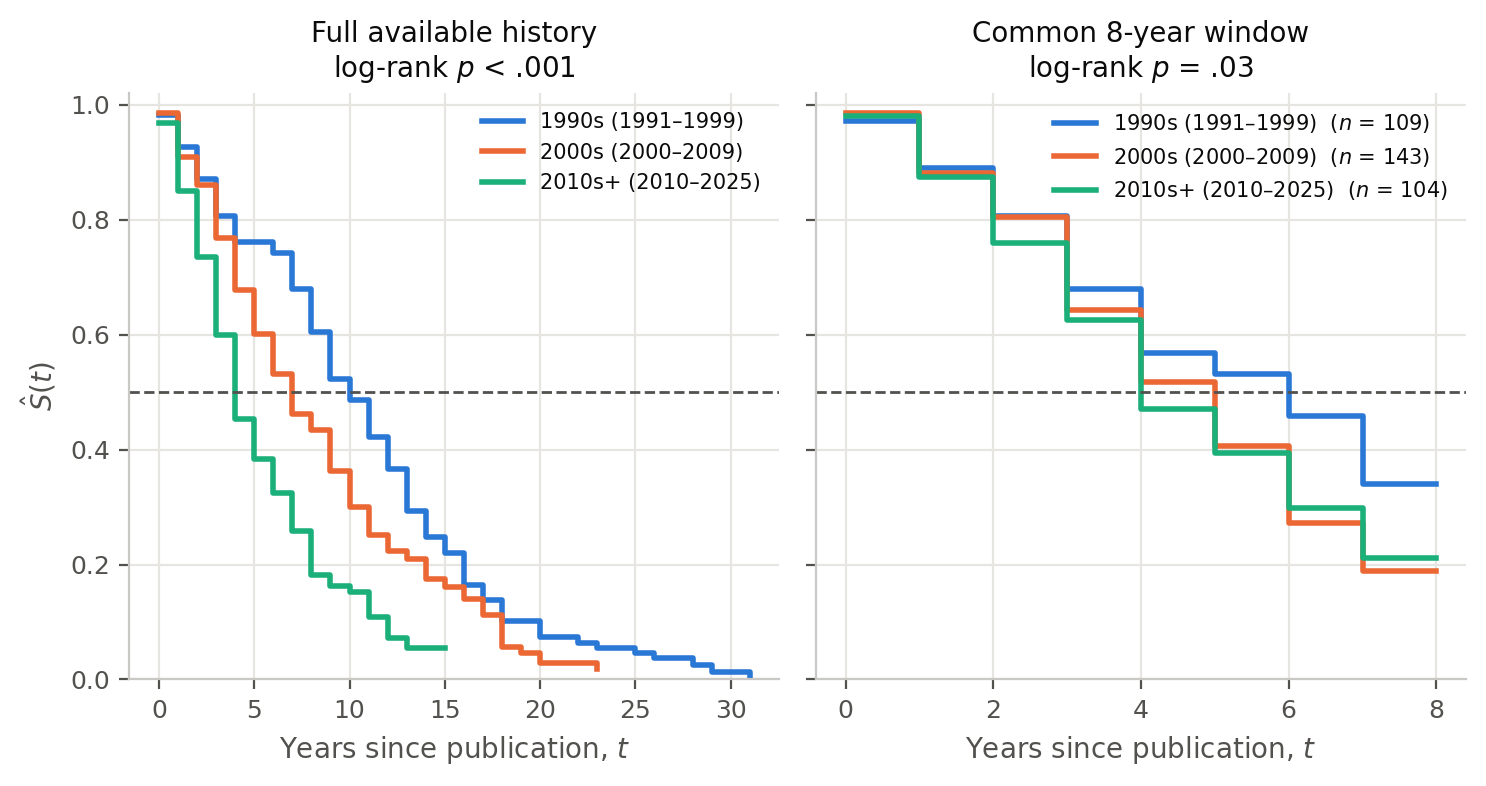
\includegraphics[width=0.8\textwidth]{figures/qd_km_era.png}
\end{figure}

\begin{table}[htbp]
\centering
\small
\caption{Association Between Author Count and Citations Across Specifications and Outcome Scales}
\label{tab:qd_specs}
\begin{tabular}{llrrr}
\toprule
Specification & Outcome scale & Multiplier & 95\% CI & $p$ \\
\midrule
Six features (Table~\ref{tab:qd_logit}) & Top decile (OR) & 1.56 & 1.10--2.19 & .011 \\
Affiliation count removed & Top decile (OR) & 1.32 & 0.98--1.77 & .071 \\
Age and authors only & Top decile (OR) & 1.32 & 0.98--1.78 & .065 \\
Six features plus topic & Top decile (OR) & 1.77 & 1.21--2.58 & .003 \\
Age, authors and topic & Top decile (OR) & 1.35 & 0.98--1.87 & .070 \\
Age and authors only & Citation count (IRR) & 1.14 & 1.00--1.29 & .048 \\
Six features & Citation count (IRR) & 1.24 & 1.06--1.45 & .007 \\
Six features plus topic & Citation count (IRR) & 1.33 & 1.15--1.54 & $<$ .001 \\
Age, authors and topic & Citation count (IRR) & 1.15 & 1.02--1.30 & .020 \\
\bottomrule
\end{tabular}
\tablenote{OR = odds ratio for membership of the top citation decile; IRR = incidence rate ratio for the citation count. All models control for log-transformed paper age. Topic is the eleven-topic NMF assignment selected under Question B. For comparison, Question A reports IRR = 1.062 ($p = .318$) and Question C reports IRR = 1.092 ($p = .006$) for the same predictor. Referenced from Question D Results.}
\end{table}

\begin{figure}[htbp]
\centering
\caption{The model does better than random guessing at spotting high-hitter papers, but not by a wide margin: bibliographic metadata alone has limited predictive power.}
\label{fig:qd_roc}
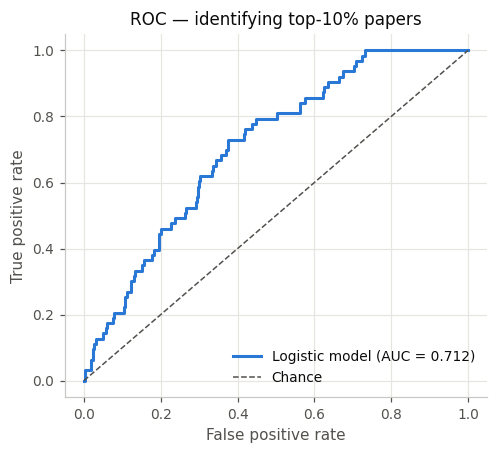
\includegraphics[width=0.5\textwidth]{figures/qd_roc.png}
\end{figure}

\begin{table}[htbp]
\centering
\small
\caption{Quantile Regression p-values by Feature and Quantile}
\label{tab:qd_qr}
\begin{tabular}{lrrrrr}
\toprule
Feature & $\tau$ = 0.10 & $\tau$ = 0.25 & $\tau$ = 0.50 & $\tau$ = 0.75 & $\tau$ = 0.90 \\
\midrule
log(age) & .000$^{*}$ & .000$^{*}$ & .000$^{*}$ & .000$^{*}$ & .000$^{*}$ \\
Number of authors & .064 & .040$^{*}$ & .040$^{*}$ & .035$^{*}$ & .031$^{*}$ \\
Number of affiliations & .198 & .762 & .469 & .291 & .167 \\
Number of keywords & .223 & .234 & .386 & .895 & .591 \\
Page length & .406 & .300 & .574 & .154 & .228 \\
Abstract length & .293 & .355 & .215 & .661 & .556 \\
\bottomrule
\end{tabular}
\tablenote{p-values from quantile regression of log(1 + citations). $^{*}$ statistically significant at p $<$ .05. Referenced from Question D Results.}
\end{table}

\subsection{Question D: characteristics considered and excluded from Part 2}\label{app:qd_excluded}

Document type has no variation, since Scopus codes every FSR record as an article. Publication year was dropped because age is an exact linear transformation of it, so a model containing both is not identified. Journal is constant in an FSR-only model. Reference-list length, funding source and open-access status are absent from the Scopus export. Author track record, abstract readability and research topic were held out for a different reason: each is the subject of Questions A, C and B respectively, and excluding them keeps Part 2 a clean test of whether the plain structural record is sufficient on its own, which is the position an editor occupies when holding only a submitted manuscript. Each is reintroduced afterwards as a cross-question check.

\end{document}
